\documentclass[a4paper]{article}
\usepackage[14pt]{extsizes}
\usepackage[utf8]{inputenc}
\usepackage[ukrainian]{babel}
\usepackage{setspace,amsmath}
\usepackage[left=20mm, top=15mm, right=15mm, bottom=15mm, nohead, footskip=10mm]{geometry}
\usepackage{tocloft}
\usepackage{indentfirst}
\usepackage{amsfonts}
\usepackage{wrapfig}
\usepackage{hyperref}
\usepackage{tabularx}

\usepackage{graphicx}
\graphicspath{}
\DeclareGraphicsExtensions{.pdf,.png,.jpg}

\usepackage{minted}


\begin{document}

\thispagestyle{empty}

\begin{center}
\textbf{Київський національний університет\\
імені Тараса Шевченка}\\
Факультет комп’ютерних наук та кібернетики\\
Кафедра обчислювальної математики\\

\vfill

\Large{\textbf{Кваліфікаційна робота}}\\
\large{\textbf{на здобуття ступеня бакалавра}}\\
за спеціальністю 113 Прикладна математика\\
на тему:\\
\Large{\textbf{Розподілені алгоритми пошуку рівноваги Неша}}
\end{center}

\vfill

\noindentВиконав студент 4-го курсу\\
Півень Денис Миколайович \hfill \underline{\hspace{4cm}}\\
\\
\\
Науковий керівник:\\
доктор фіз.-мат. наук, професор\\
Семенов Володимир Вікторович \hfill \underline{\hspace{4cm}}

\begin{flushright}
\begin{minipage}{.5\textwidth}
Засвідчую, що в цій роботі немає запозичень з праць інших авторів без відповідних посилань.\\
\\
\\
Студент \hfill \underline{\hspace{4cm}}\\
\\
\\
Роботу розглянуто й допущено до захисту на засіданні кафедри обчислювальної математики\\
<<\underline{\hspace{5mm}}>>\underline{\hspace{4.5cm}}202\_р.,\\
протокол №\underline{\hspace{5mm}}\\
Завідувач кафедри\\
С. І. Ляшко \hfill \underline{\hspace{4cm}}
\end{minipage}
\end{flushright}

\vfill

\centerline{\textbf{Київ --- 2022}}
\clearpage


\section*{Реферат}

Обсяг роботи 25 сторінок, 16 джерел посилань, 1 додаток.

Ключові слова:

РОЗПОДІЛЕНИЙ АЛГОРИТМ, РІВНОВАГА НЕША, АГРЕГАТИВНА ГРА, ДИНАМІКА НЕПЕРЕРВНОГО ЧАСУ, МЕРЕЖЕВА ГРА, РОЗПОДІЛЕНЕ НАВЧАННЯ, АЛГОРИТМ ПРОКСИМАЛЬНОЇ ТОЧКИ.

Об’єкт дослідження --- розподілені алгоритми пошуку рівноваги Неша.

Мета роботи --- розробка розподілених алгоритмів на основі класичних сучасних та перевірка ефективності їх роботи.

Результати: було сформульовано, реалізовано та протестовано 3
розподілених алгоритми.

\clearpage


\renewcommand\cftsecdotsep{\cftdot}
\cftsetpnumwidth{9pt}
\tableofcontents
\clearpage

\section{Вступ}
Протягом життя ми постійно взаємодіємо з іншими людьми. Маленькі діти, намагаючись добитися того, щоб батьки купили вподобану цукерку, часто шантажують батьків своїми слізьми. Приймаючи рішення заплакати, дитина ризикує — він не знає, як будуть поводитися тато з мамою. У трохи більш дорослому віці абітурієнти, які вибирають виш, приймають складне рішення в тому, до яких університетів подати документи. Помилка може коштувати дорого: при неправильній стратегії можна опинитися в слабкому університеті або взагалі залишитися без заповітного студентського квитка. Закінчивши виш, юнаки й дівчата починають шукати роботу. Перед інтерв'ю з роботодавцем вони переглядають статті в інтернеті в тому, що можна і чого не можна говорити на інтерв'ю, — вони намагаються знайти найкращу стратегію своєї поведінки, виходячи з очікувань компанії, в яку вони влаштовуються. Всі ці ситуації об'єднує те, що рішення, які приймають люди, впливають на інших. Пошук найкращої стратегії є не тривіальною задачею, як для дитини, так і для дорослого. На жаль не всі діють за принципами теорії прийняття рішень, теорії ігор чи просто аналітично розв'язують поставлену перед ними проблему.

На мій погляд, найбільший вплив проблема пошуку оптимального рішення відіграє в економіці. На сьогодні, згідно з економічною теорією, конкурентна рівновага є оптимальним станом економіки, і відхилення від нього пов'язано зі зниження її ефективності. Одна з можливих причин цього відхилення — зміна ціни товару в результаті дій виробника або споживача товару, який контролює значну частку в загальному обсязі продажів. Велика частина реальних ринкових продажів олігополії. В той час, як окремий споживач не має ринкової влади і його вплив у загальному обсязі продажів складає соті відсотка, найбільший виробник на таких ринках забезпечує не менше 10\% від загального споживання. Дослідження математичних моделей і оцінка очікуваного відхилення від стану конкурентної рівноваги для різних типів олігополії становлять великий інтерес. Типовим підходом до кількісної характеристики умов досконалої конкуренції та до оцінки очікуваного відхилення є порівняння конкурентної рівноваги з рішенням гри, яка описує олігополістичну конкуренцію.

Метою даної роботи є дослідження постановки математичної моделі проблеми пошуку рівноваги Неша у мережево агрегативних іграх та проведення чисельних експериментів алгоритмів пошуку її оптимального рішення.


\clearpage

\section{Опис алгоритмів}
\subsection{Умова задачі}
У теорії ігор агрегативна гра — це гра, в якій виграш кожного гравця є функцією власної стратегії гравця та сукупності стратегій усіх гравців. Вперше концепція була запропонована Нобелівським лауреатом Рейнхардом Сельтеном в 1970 році, який розглянув випадок, коли сукупність є сумою стратегій гравців. У нашому випадку гра є мережевою, тобто кожен гравець спілкується з іншими гравцями та отримує інформацію про їхні стратегії. Гра відбувається покроково, спочатку всі гравці обирають випадкову стратегію, далі вони повідомляють її своїм <<знайомим>> та отримують інформацію про їхні стратегії, змінюють свою стратегію деяким чином, далі процес продовжується доки кожному гравцю буде непотрібно змінювати стратегію.

Агрегативна гра містить у собі $n$ гравців проіндексованих як $N = \{1, 2, ... , n\}$, де кожен гравець $i$ має обрати стратегію $x_i \in X_i \subseteq \mathbb{R}^m$ з ціллю мінімізувати функцію витрат $f_i (\mathbf{x}_i, \mathbf{\bar{x}}),~f_i: \mathbb{R}^n \times \mathbb{R}^n \rightarrow \mathbb{R} \cup \{ \infty \}$, де $\mathbf{\bar{x}} = \frac{1}{n} \sum_{j=1}^{n} \mathbf{x}_j$

\subsection{Алгоритм динаміки неперервного часу~\cite{Article1}}\label{alg1}
Надалі буде розглянуто напівдецентралізовану динаміку неперервного часу для обчислення рівноваги в класі агрегатних ігор. Зокрема, схему де децентралізована динаміка прогнозованого градієнта визначає цілісний закон контролю. Буде доведено глобальну експоненціальну збіжність запропонованої динаміки до сукупної рівноваги. Буде виведено достатню умову глобальної конвергенції, позиціоновану в рамках сучасної літератури про агрегатні ігри та показано, що це покращує визнані результати.

Більшість алгоритмів розглядають дискретну динаміку часу, що за відповідних технічних припущень і достатніх умов щодо даних задачі, сходяться до рівноваги гри. Елегантний підхід фактично полягає у характеристиці бажаної рівноваги, формулює задачу з нерухомою точкою, яка вирішується за допомогою відповідної нелінійної дискретної динаміки із гарантованою глобальною асимптотичною конвергенцією.

З іншого боку, лише декілька внесків розглядали проблему обчислення рівноваги через динаміку неперервної роботи, наприклад \cite{Cite22}, \cite{Cite21}. Одна з причин полягає в тому, що у випадку неперервного часу, виникають проблеми з оптимальним рішенням.

\begin{figure}[]
\center{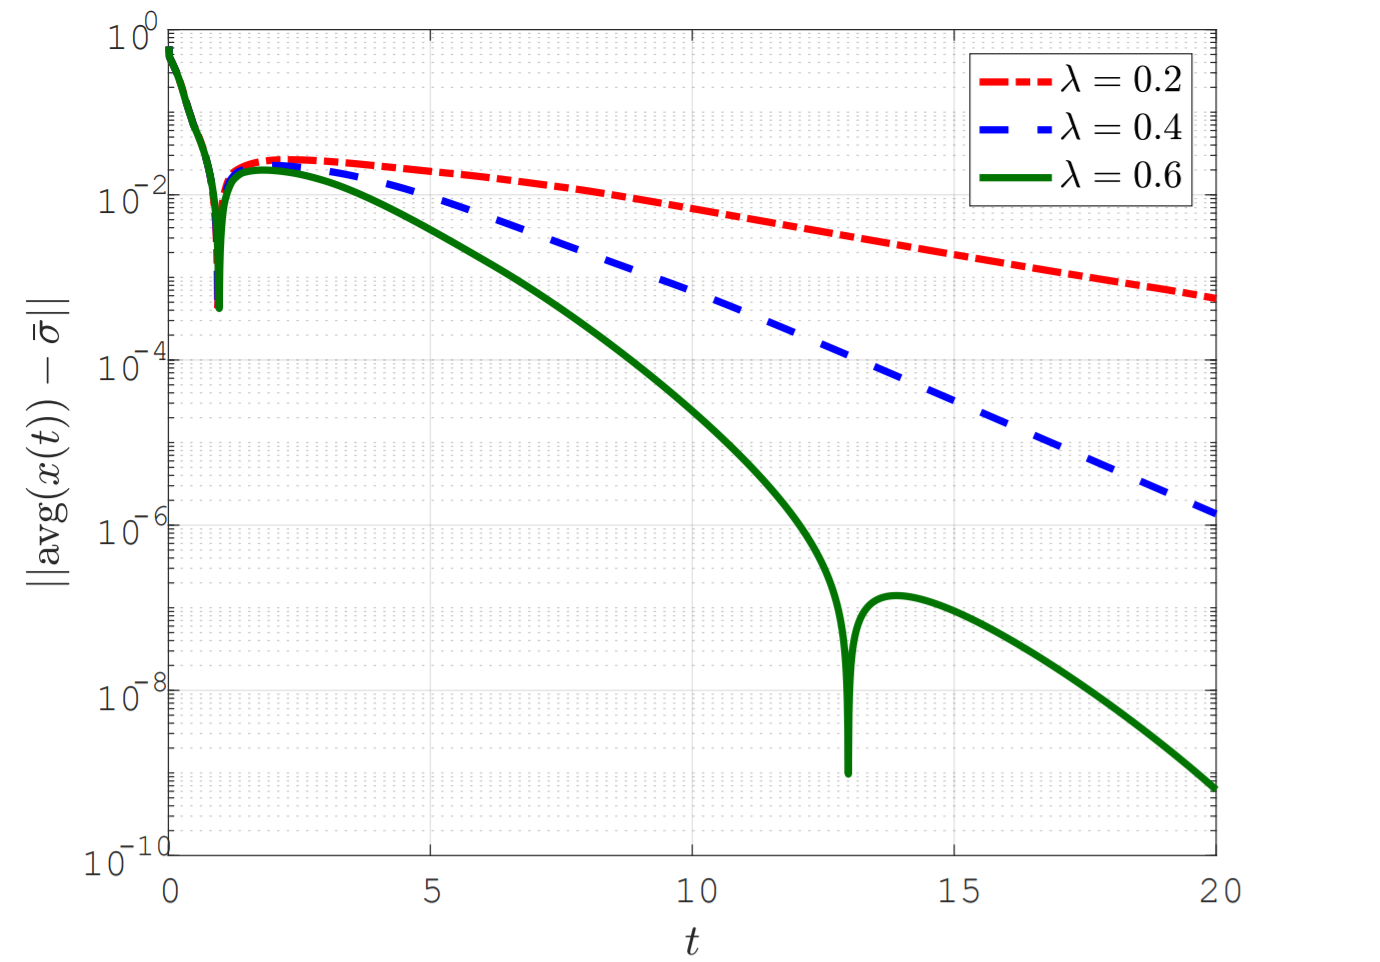
\includegraphics[scale=0.5]{plot11.png}}
\caption{Відстань між середніми стратегіями досліду та рівноваги.}
\label{ris:plot11}
\end{figure}

Для кожного гравця $i \in N$ функція витрат $f_i$ має вигляд:
\begin{equation}
f_i(x_i,\sigma) = g_i(x_i)+(C\sigma)^\mathrm{T}x_i\\
\end{equation}
де функція $g_i:\mathbb{R}^n \rightarrow \mathbb{R}$ двічі неперервно диференційована та сильно опукла на множині $X_i$, з $C \in \mathbb{R}^{n \times n}$

\subsubsection*{Алгоритм}
З метою досягнення рівноваги пропонується скористатись неперервною динамікою часу:
\begin{align}
\dot x_i &= x_i-\partial g_i(x_i)-C\sigma, \quad \forall i \in N\\
\dot \sigma &= \lambda\left(-\sigma+\mathbf{\bar{x}}\right)\label{lambda} 
\end{align}
де
\begin{equation}
\partial g(x) = \left\{ v \in \mathbb{R}^m~|~g(z)\geq g(x)+v^\mathrm{T}(z-x),\forall z \in \left\{x\in \mathbb{R}^m~|~g(x)< \infty\right\}\right\}
\end{equation}
субдиференціальний набір значень, якщо $g$ диференційована по $x$, то $\partial g(x) = \{\nabla g(x)\}$, та $\lambda>0$ вільний параметр.  

Зазначимо, що структура обчислень та обміну інформацією є напівдецентралізованою: гравці виконують обчислення і не обмінюються інформацією між собою, в той час, як центральний блок управління, який не бере участі в грі, збирає середнє значення їх рішень $\mathbf{\bar{x}}(t)$ та передає сигнал $\sigma(t)$ гравцям.

\begin{figure}[]
\center{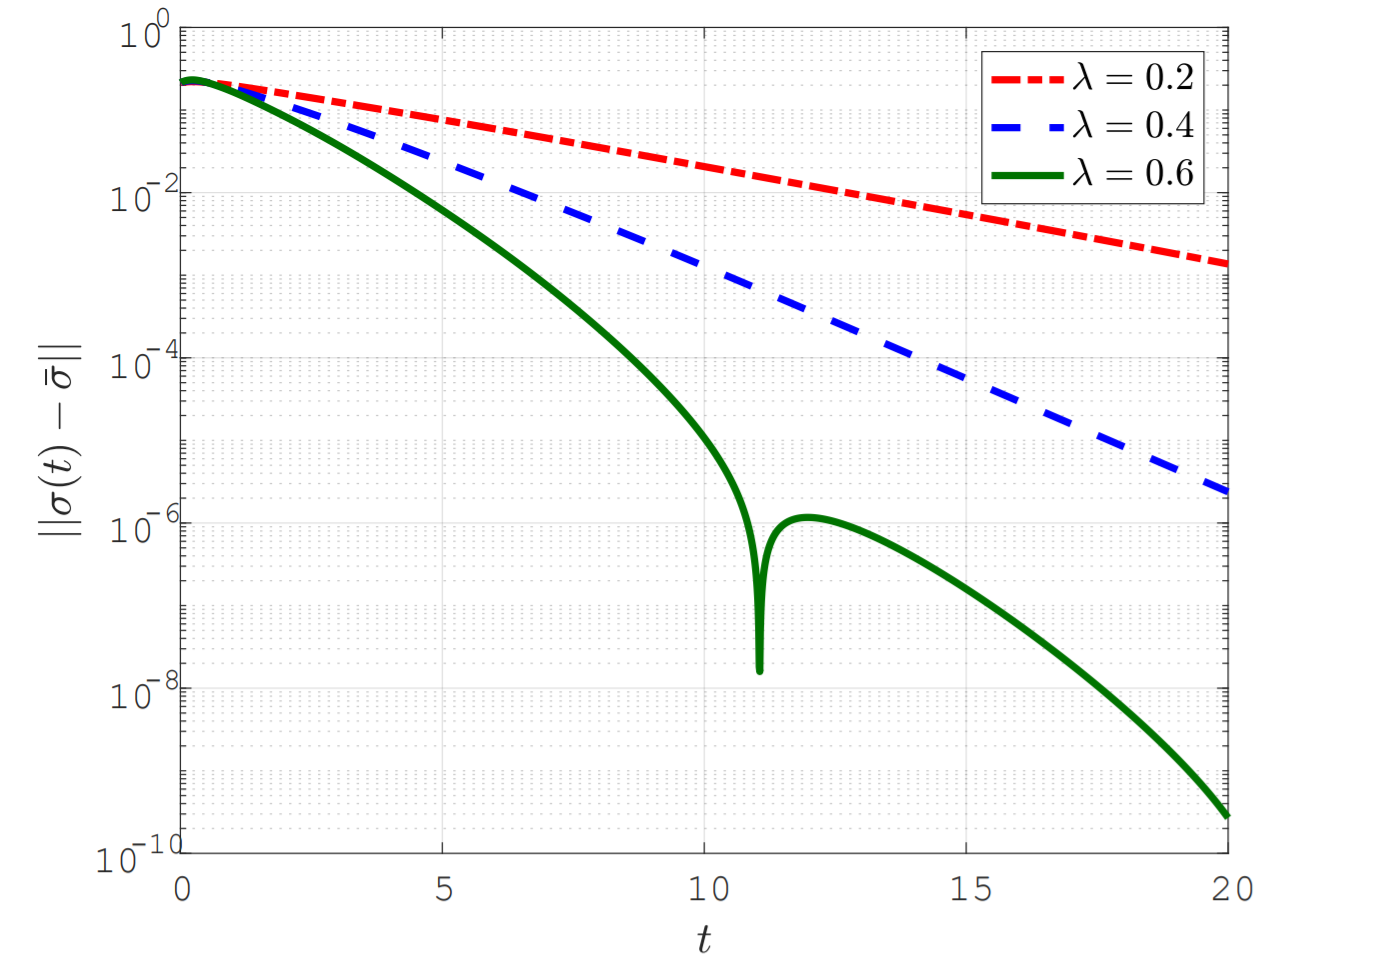
\includegraphics[scale=0.5]{plot22.png}}
\caption{Відстань між інтегральним керуючим сигналом та його рівновагою.}
\label{ris:plot22}
\end{figure}

\subsubsection{Числове моделювання}
Одною з основних областей застосування агрегатних ігор є
управління попитом, де гравці є споживачами або виробниками електроенергії, чия функція витрат залежить від середнього показника попиту електроенергії, через загальну ціну на неї. Наприклад, у [\ref{Cite22}, розділ 5.2], функція індивідуальних витрат кожного гравця обирається як:
\begin{equation}
    f_i(x_i,\sigma)=\frac{1}{2}l_i\|x_i-x_i^*\|^2+(a\sigma+b)^\mathrm{T}x_i~,
\end{equation}
де $x_i^* \in \mathbb{R}$ досяжна змінна, параметр $l_i>0$, параметри $a \in \mathbb{R}$ та $b \in \mathbb{R}^n$.

Для досліду були взяті наступні значення параметрів: $N=100, a=1,\\ b=0.5, X_i=[0.25, 0.75], x_i^* \sim U(0,1)$ та $l_i = 1.5, ~\forall i\in N$.

Розглянуто задачі для трьох випадків $\lambda=0.2, \lambda=0.4, \lambda=0.6$, графіки ілюструють відстань між середньою стратегією досліду та середньою стратегією рівноваги в часі $\|\mathbf{\bar{x}}(t) - \bar{\sigma}\|$ (Рис.\ref{ris:plot11}), а також відстань між інтегральним керуючим сигналом $\sigma(t)$ та його рівновагою $\bar{\sigma}$ (Рис.\ref{ris:plot22}).

Згідно з попередніми дослідженнями коефіцієнт посилення $\lambda$ з (\ref{lambda}) може помітно пришвидшити зближення до рівноваги, але тільки до критичного значення, вище якого можуть виникати коливання.
\subsubsection*{Висновок}
В контексті агрегатних ігор, інтегральна динаміка з неперервним часом, напівдецентралізованими обчисленнями та обміном інформацією може забезпечити глобальну асимптотичну збіжність до агрегатних рівноваг за умови посилення контролю обраного належним чином. Майбутні дослідження будуть зосереджені на розширенні збіжності та аналізі на випадок загальних мережевих ігор, можливо, з обмеженням та різними технічними припущеннями.

\clearpage
\subsection{Лінійно збіжний алгоритм \cite{Article2}}\label{alg2}
Новий розподілений алгоритм спільно використовує ідеї алгоритму консенсусу та умовного проєкційного спуску \cite{Cite1}. За сильно монотонного припущення про псевдоградієнтне відображення, доведемо запропонований алгоритм із фіксованими розмірами кроків, що лінійно збігається до рівноваги Неша. Потім теоретичні результати перевіримо числовими експерименти.

\subsubsection{Мережева агрегативна гра}
Розглянемо набір з $n$ гравців, проіндексованих як $N = \{1, 2, ... , n\}$.
В агрегативній грі функція витрат гравця $i$, $f_i (\mathbf{x}_i
, \mathbf{\bar{x}})$ залежить від власної дії $\mathbf{x}_i \in X_i \subset \mathbb{R}^p$ та сукупності дій гравців $\mathbf{\bar{x}} = \frac{1}{n} \sum_{i=1}^{n} \mathbf{x}_i$ . Завдання гравця $i$ в АГ полягає в мінімізації його витрат: $f_i (\mathbf{x}_i, \mathbf{\bar{x}})$ де $\quad\mathbf{x}_i \in X_i$, a $ \mathbf{x}_j$, $j \neq i$, $j \in N$ фіксовані, та пошук рівноваги Неша відбувається для всіх гравців.
Взаємодія гравців між собою описується матрицею ваг $W = \{w_{ij}\}_{n\times n}$ де $w_{ij} > 0$ якщо гравці спілкуються, та $w_{ij} = 0$ в іншому випадку.
\subsubsection*{Алгоритм}
Спочатку для кожного гравця $i \in N$ обираємо стратегію $\mathbf{x}_i^0 \in X_i$ випадковим чином та $\mathbf{v}_i^0=\mathbf{x}_i^0$.

Повторюємо наступну процедуру для всіх гравців $i \in N$ допоки не зійдемось. 
\begin{align}
\mathbf{\hat{v}}^{k+1}_i &= \sum_{j=1}^{n} w_{ij}\mathbf{v}^k_i,\\
\mathbf{\hat{x}}^{k+1}_i &= \prod_{X_i} \left[\mathbf{x_i^k-\alpha F_i\left(\mathbf{x_i^k},\mathbf{\hat{v}}^{k+1}_i\right)}\right],\\
\mathbf{x}^{k+1}_i &= \mathbf{x}^{k}_i + \beta\left(\mathbf{\hat{x}}^{k+1}_i-\mathbf{x}^{k}_i\right),\\
\mathbf{v}^{k+1}_i &= \mathbf{\hat{v}}^{k+1}_i + \mathbf{x}^{k+1}_i-\mathbf{x}^{k}_i.
\end{align}
де $\alpha$ оберемо достатньо малим, щоб послідовність $\{\mathbf{x}^k\}_{k\in \mathbb{N}}$ збігалась до фіксованої точки $\mathbf{x}^*$, $\mathbf{v}_i$ локальний вектор, що змінюється в залежності від дій сусідів, $\alpha > 0$ та $\beta \in (0,1]$ розмір кроку.

\begin{figure}[]
\center{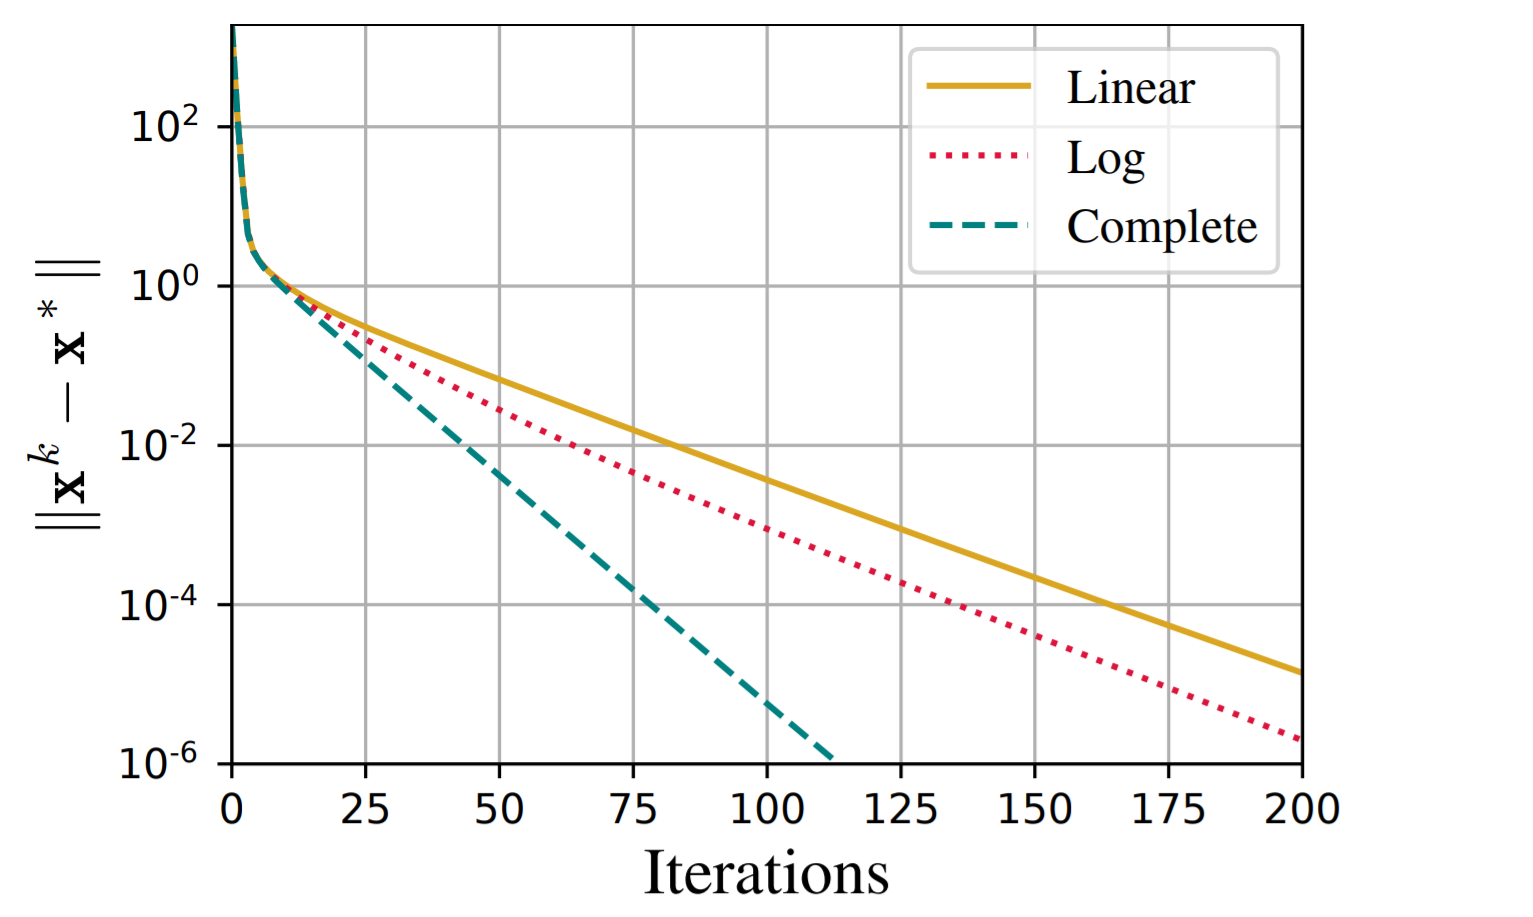
\includegraphics[scale=0.4]{plot1.png}}
\caption{Траєкторії розриву субоптимальності у різних топологіях мережі.}
\label{ris:plot1}
\end{figure}

\subsubsection{Числовий експеримент}
Розглянемо $n = 20$ фірм, що контролюють $L = 10$ локацій, кожній фірмі $i$ потрібно обрати її продукцію $g_{il}$, та знижки $s_{il}$ на локації $l$.

Ціну продукції фірми $i$ на локації $l$ позначимо як $c_{il}(g_{il})$ та визначимо як
$c_{il}(g_{il}) = a_{il}g_{il} + b_{il}g_{il}^2,$ де $a_{il}$ та $b_{il}$ параметри фірми $i$.

Дохід фірми $i$ на локації $l$ є $s_{il}p_{l}(s_l)$ де $s_l = \sum_{i=1}^{n} s_{il}$ загальна знижка локації та $p_{l}$ відповідна функція ціни.

Функція ціни $p_l$ є функцією резервного попиту та визначається як $p_l(s_l) = d_l - s_l,$ де $d_l$ це параметр локації $l$.

Місткість продукції фірми $i$ на локації $l$ запишемо як $cap_{il}$. Припускаючи, що плата за транспортування між двома локаціями нульова, тоді проблема для фірми $i$ виглядає так:
\begin{align}
&\sum_{l=1}^L \left[c_{il}(g_{il}) - s_{il}\cdot p_l(s_l)\right] \rightarrow min\\
&g_{il},s_{il}\geq 0, \quad g_{il} \leq cap_{il},\\
&\sum_{l=1}^L g_{il} = \sum_{l=1}^L s_{il}.
\end{align}
У симуляції було покладено $a_{il} \sim U(2,12), b_{il} \sim U(2,3), d_l \sim U(90,100)$ та $cap_{il} = 500$ для $i = 1, ..., n$ та $l = 1, ..., L.$ де $U(u_1,u_2)$ рівномірний розподіл на інтервалі $[u_1, u_2]$.

Алгоритм було розглянуто для трьох випадків:
\begin{itemize}
\item \textit{Linear}: гравець $i$ спілкується з гравцями mod$(i+11j,n)+1, 0 \leq j < n/11.$
\item \textit{Log}: гравець $i$ спілкується з гравцями mod$(i+2^j,n)+1, 0 \leq j < \mathrm{log}_{2}~n.$
\item \textit{Complete}: кожен гравець спілкується зі всіма.
\end{itemize}

\begin{figure}[]
\center{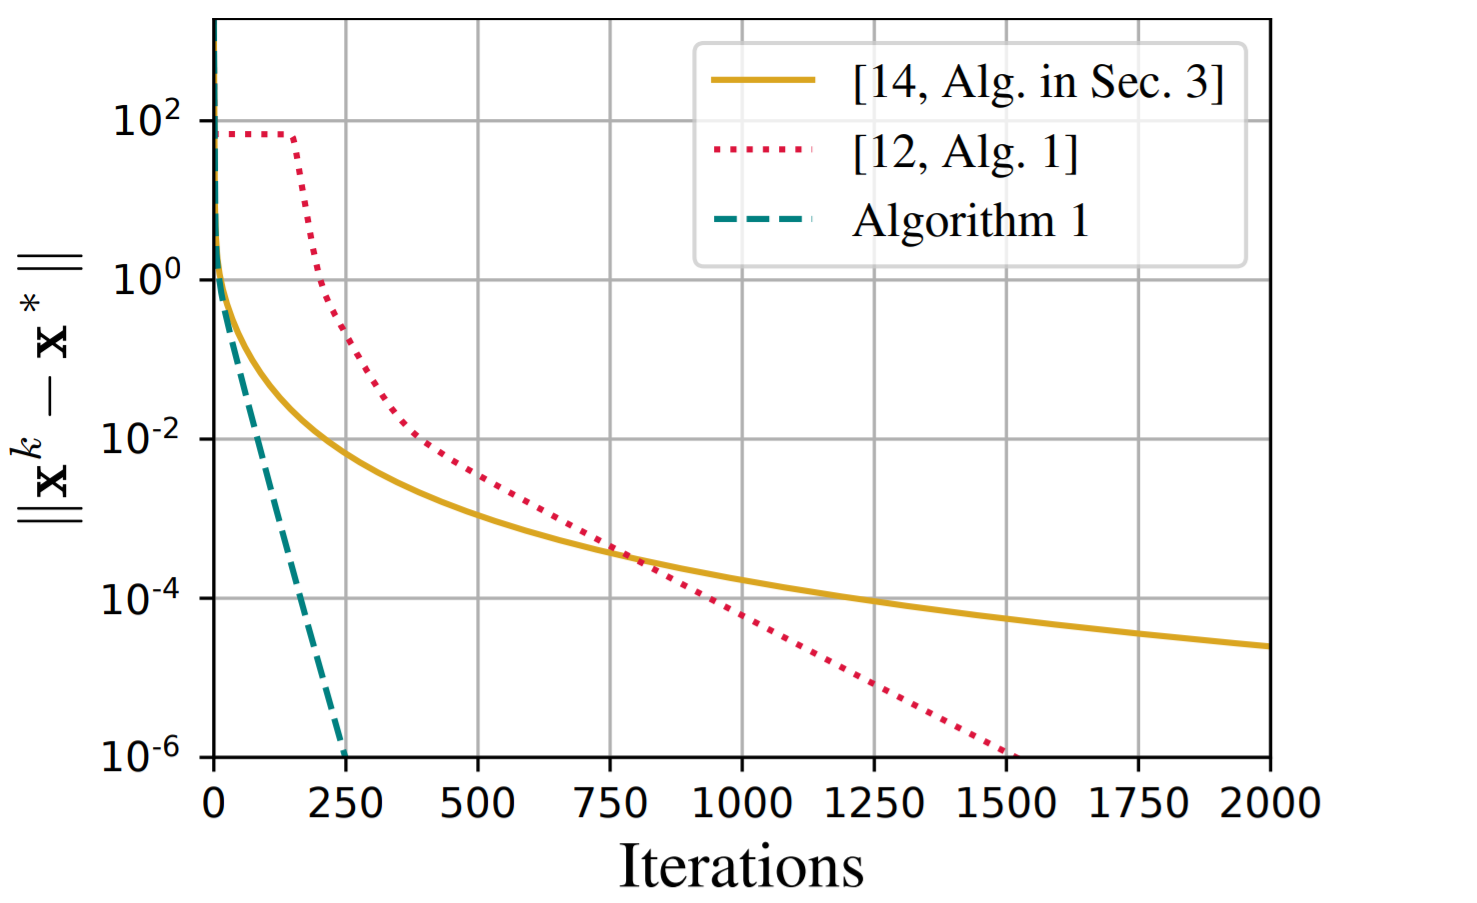
\includegraphics[scale=0.4]{plot2.png}}
\caption{Порівняння різних алгоритмів.}
\label{ris:plot2}
\end{figure}

Матриця ваг $W = \{w_{ij}\}$ задається так
\begin{eqnarray}
w_{ij} =
\begin{cases}
0, & (i,j) \notin E \\
\delta, & (i,j) \in E, i\neq j\\
1-\delta \cdot d(i), &  i = j
\end{cases}
\end{eqnarray}
де $d(i)$ число гравців, що спілкуються с гравцем $i$, та $\delta = 0.5/\mathrm{max}_i{d(i)}$, та $E$ множина пар, що спілкуються між собою. Рис.~\ref{ris:plot1} описує траєкторії субоптимального розриву $||\mathbf{x}^k - \mathbf{x}^*||$ для різної кількості ітерацій, для трьох мережевих топологій. Всі топології починаються з однієї точки з оптимальним розміром кроку. Можна бачити, як алгоритм лінійно збігається для різних топологій.

Щоб знайти оптимальне значення коефіцієнта $\alpha$ фіксуємо різні значення коефіцієнта $\beta$, приклад лінійної топології наведено у таблиці.

\begin{wraptable}{l}{0.65\linewidth}
\begin{tabular}{ | c | c | c | c | c | c | c | }
\hline
$\beta$&& 0.8&0.85 &0.9 &0.95 &1 \\\hline
$\alpha$&&0.108 &0.092 &0.096 &0.090& 0.087\\\hline
$\varepsilon _{200} (\times 10^{-5})$&& 1.615&1.622 & \textbf{1.418}&1.512 &1.591\\
\hline
\end{tabular}
\end{wraptable}
Порівняємо описаний та \cite{Cite2}, \cite{Cite3} алгоритми, з яких перший призначений для ігор, де функції витрат залежать від дій загалом, а останній призначений для мережевої агрегативної гри, але лише зі зменшенням розмірів кроків. Рис.~\ref{ris:plot2} показує, що описаний алгоритм перевершує інші. Алгоритм \cite{Cite2} застряє у початковій фазі, яка обумовлена властивістю кожного гравця робити помилкову оцінку дій сусідів. Що стосується алгоритму в \cite{Cite3}, то він використовує зменшувані розміри кроків та також поступається описаному алгоритму.

\subsubsection*{Висновок}
Вище був запропонований повністю розподілений алгоритм для мережевої агрегативної гри за ненаправленим зв’язком мережі. Коли мережева агрегативна гра є сильно монотонною та має неперервне відображення Ліпшіца. Доведено, що алгоритм з фіксованими розмірами кроків збігається лінійно до рівноваги Неша.  У подальшій роботі будуть розглянуті лінійно збіжні алгоритми для мережевих агрегативних ігор через мережі спрямованого зв'язку або мережі, що змінюються з часом.

\subsection{Алгоритм розподіленого навчання \cite{Article3}}\label{alg3}
У стохастичних задачах рівноваги за Нешем для гравців природно бути неінформованими про їх середовище та мати багатовимірні невідомі параметри у своїх моделях. Цей алгоритм зосереджується на локально пов'язаних мережевих іграх, де мета кожного раціонального гравця підлягає сукупному впливу на його сусідів, алгоритм розроблено на основі ітерації проксимальної точки та звичайної оцінки методом найменших квадратів, де кожен гравець багаторазово оновлює локальні оцінки сусідів, приймає найкраще рішення за можливих, з урахуванням поточних оцінених параметрів отримує реалізовані об'єктивні значення, і вивчає невідомі параметри. Використовуючи теорему Роббінса-Зігмунда та закон великих відхилень для M-оцінок, встановлюється майже впевнену збіжність
запропонованого алгоритму розв'язання стохастичних задач рівноваги за Нешем, коли розміри кроків оновлення зменшуються з належною швидкістю.

Розподілений алгоритм навчання, який гарантує майже впевнену збіжність до стохастичної рівноваги Неша в локально пов’язаних мережевих іграх з невідомими параметрами. Припускаємо, що після того, як усі гравці визначають свої рішення, кожен гравець може спостерігати за своїми власними рішеннями та усвідомлювати об'єктивну цінність рішень, прийнятих його сусідами. На кожній ітерації кожен гравець вибирає своє рішення, зазначене розв’язком його доповненої параметризованої функції найкращої відповіді за поточними оцінками параметрів разом із деяким випадковим вектором дослідження. Потім кожен гравець отримує зворотний зв’язок про об’єктивні значення та рішення сусідів і оновлює свої параметри за допомогою звичайної оцінки найменших квадратів. Крім того, на відміну від більшості існуючих алгоритмів, які користуються скорочувальними ітераціями в динаміці пошуку рівноваги Неша, оператор ітерації з фіксованою точкою задовільняє лише (квазі)нерозширеність через налаштування часткової інформації. Використовується теорема Роббінса-Зігмунда, встановлюється основна теорема збіжності для запропонованого алгоритму та обговорюються умови, необхідні для забезпечення збіжності розв'язків. Отримується верхня межа для швидкості асимптотичної збіжності та обговорюється правильний вибір розмірів кроків, щоб гарантувати збіжність.

\subsubsection{Формулювання локально з’єднаних мережевих ігор}
Розглядаємо гру, в яку грає група зацікавлених гравців, індексована $\mathcal{N} := \{1, . . . , N\}$, взаємодії яких визначаються базовою мережею зв'язку $\mathcal{G} = (\mathcal{N} , \mathcal{E})$. Використовуємо $(i, j)$ для позначення спрямованого ребра, у якого гравець $i$ є хвостом, а $j$ --- головою. Хоча кожне ребро $e \in \mathcal{E}$ допускає певний напрямок, зв'язок через ребро $e$ ненаправлений, тобто кожен гравець $i$ може надсилати повідомлення обом його внутрішнім сусідам $\mathcal{N}_i^+ := \{j \in \mathcal{N}\, | \,(j, i) \in \mathcal{E}\}$ та зовнішнім сусідам $\mathcal{N}_i^- := \{j \in \mathcal{N}\, |\, (i, j) \in \mathcal{E}\}$, потужності яких позначаються $\mathcal{N}_i^+$ та $\mathcal{N}_i^-$ відповідно.

Мета кожного гравця $i$ полягає в тому, щоб мінімізувати ціль очікуваної вартості, визначену $\mathbb{J}_i(x_i; x_i^+, w_i^*) := \mathbb{E}[J_i(x_i; s_i(x_i^+; \xi_i, w_i^*))]$, що залежить від його власного рішення $x_i \in \mathbb {R}^{n_i}$ та рішення його внутрішніх сусідів $x_i^+ := [x_j]_{j\in \mathcal{N}_i^*}$. Варто згадати, що $х_i^*$ розглядаються як параметричні входи $\mathcal{J}_i$.

Використаємо $s_i$ для позначення сусідньої агрегатної функції: $$s_i(x_i^+; \xi_i, w_i^*) := w_{ii}^* + \sum_{j\in \mathcal{N}_i^+} w_{ji}^{*T} x_j + \xi_i,$$ де $w_{ii}^* \in \mathbb{R}$ та $w_{ji}^* \in \mathbb {R}^{n_j}$ — деякі постійні параметри, також введемо випадкову величину $\xi_i: \Omega \rightarrow \mathbb{R}$ що описує невизначеність в $s_i$. Рішення $x_i$, прийняте гравцем $i$, підпорядковується набору локальних обмежень $X_i \subseteq \mathbb {R}^{n_i}$. 

Далі визначимо: $$w_{i}^{*}:=\left[w_{j i}^{*}\right]_{j \in\{i\} \cup \mathcal{N}_{i}^{+}},\: w^{*}:=\left[w_{i}^{*}\right]_{i \in \mathcal{N}},\: n:=\sum_{i \in \mathcal{N}} n_{i},\: n_{i}^{+}=\sum_{j \in \mathcal{N}_{i}^{+}} n_{j},\: \mathcal{X}:=\prod_{i \in \mathcal{N}} \mathcal{X}_{i}$$ Допустимий набір параметрів гравця $i$ позначається $\mathcal{W}_{i}$, та $w_{i}^{*} \in \mathcal{W}_{i}$. Загалом, локальна проблема стохастичної оптимізації гравця $i$ може формально записати так:
\begin{equation}\label{sne}
    \operatorname{minimize}_{x_{i} \in \mathcal{X}_{i}} \mathbb{J}_{i}\left(x_{i} ; x_{i}^{+}, w_{i}^{*}\right)
\end{equation}

Укладаючи часткові градієнти $\partial_{x_{i}} \mathbb{J}_{i}\left(x_{i} ; x_{i}^{+}, w_{i}^{*}\right)$ можемо побудувати псевдоградієнтний оператор $\mathbb{F}_{w^{*}}: \mathcal{X} \Rightarrow \mathbb{R}^{n}$ як $\mathbb{F}_{w^{*}}: x \mapsto\left[\partial_{x_{i}} \mathbb{J}_{i}\left(x_{i} ; x_{i}^{+}, w_{i}^{*}\right)\right]_{i \in \mathcal{N}}$. 
Цей оператор грає значну роль у регулюванні різних видів ігор, аналізі властивостей множин рішень, і т.п. Ігри з максимально монотонним псевдоградієнтом $\mathbb{F}_{w^{*}}$ називають монотонними іграми. Щоб обчислити рівновагу Неша для задачі потрібно розв'язати відповідну узагальнену варіаційну нерівність: знайти пару векторів $\left(x^{*}, g^{*}\right)$ такий, що $x^{*} \in \mathcal{X}$ та $g^{*} \in \mathbb{F}_{w^{*}}\left(x^{*}\right)$ та $\left(x-x^{*}\right)^{T} g^{*} \geq 0, \forall x \in \mathcal{X}$. Задачу можна переписати через необхідні умови оптимальності задачі (\ref{sne}):
\begin{equation}
    \mathbf{0} \in \partial_{x_{i}} \mathbb{I}_{i}\left(x_{i} ; x_{i}^{+}, w_{i}^{*}\right)+N_{\mathcal{X}_{i}}\left(x_{i}\right), \forall i \in \mathcal{N},
\end{equation}
Коротко обговоримо один приклад подібної задачі.
\subsubsection*{Приклад}
Існує скінченна множина гравців, індексованих $i = 1, . . . , N$, кожен з яких створює скалярну невід’ємну обмежену стратегію $x_i$ щоб оптимізуючи його квадратичну мету $J_{i}(x_{i} ; x_{i}^{+}):=\frac{1}{2}(x_{i})^{2}+(K_{i} \sum_{j \in \mathcal{N}_{i}^{+}} w_{i j} x_{j}-a_{j}) x_{i} \text {, де } K_{i}, a_{i} \in \mathbb{R}$, та $w_{ij}$ вказує на вплив рішення гравця $j$ на цільову функцію гравця $i$. Ця модель була застосована для дослідження різних економічних умов, включаючи приватне надання суспільні блага та ігри з локальною взаємодоповнюваністю, але глобальною замінністю.

\subsubsection{Розподілене рішення за допомогою алгоритму проксимальної точки з точними параметрами}
Починаємо з пропозиції розподіленого рішення для проблеми пошуку рівноваги за Нешем з точно заданими параметрами. Алгоритм є реалізацією схеми з фіксованою точкою, може здійснюватися розподіленим і незалежним чином, кожен гравець приймає рішення на основі рішень інших гравців з останньої ітерації. Однак, властивості збіжності залежать від скоротливості їхніх ітерацій з фіксованою точкою, що вимагає додаткових закономірностей щодо цілей та мережевих структур.

Дано скінченновимірний максимально монотонний оператор $A$, резольвента $J_{A}:=(I+A)^{-1}$  є твердо нерозширювальною. Отримуємо наступний прототип ітерації $x^{(k+1)}:=x^{(k)}+\gamma^{(k)}\left(J_{A} x^{(k)}-x^{(k)}\right)$, який генерує послідовність, що збігається до точки в $\operatorname{Zer}(A)$, нульовому наборі $A$. Тут $\left(\gamma^{(k)}\right)_{k \in \mathbb{N}}$ задовольняє умови $\gamma^{(k)} \in[0,1]$ та $\sum_{n \in \mathbb{N}} \gamma^{(k)}\left(1-\gamma^{(k)}\right)=+\infty$

Кожному гравцю $i \in \mathcal{N}$ дамо локальну оцінку $y_{i}^{j}$ для рішення кожного з його внутрішніх сусідів $j \in \mathcal{N} _{i}^{+}$. Далі використовуємо $y_{i}^{i}$ для позначення локального рішення гравця $i$, де $y_{i}^{+}:= [y_{i}^{j}]_{j \in \mathcal{N}_{i}^{+}}$ стек локальних оцінок рішень його внутрішніх сусідів, та $y_{i}^{-}:= [y_{j}^{i}]_{j \in \mathcal{N}_{i}^{-}}$ стек локальних оцінок рішень його зовнішніх сусідів. Нехай $y_{i}:=[y_{i}^{i} ;[y_{i}^{j}]_{j \in \mathcal{N}_{i}^{ +}}]$ та $y:=[y_{i}]_{i \in \mathcal{N}}$. Допустима область вектора стека $y_{i}$ визначається як $\tilde{\mathcal{X}}_{i}:=\mathcal{X}_{i} \times \mathbb{R}^{ n_{i}^{+}}$. Нехай $\tilde{\mathcal{X}}:=\prod_{i \in \mathcal{N}} \tilde{\mathcal{X}}_{i} \subseteq \mathbb{R}^{\tilde{ n}}$, де $\tilde{n}:=n+\sum_{i \in \mathcal{N}} n_{i}^{+}$. З введенням локальних оцінок ми можемо побудувати розширений псевдоградієнт $\tilde{\mathbb{F}}_{w^{*}}: \tilde{\mathcal{X}} \Rightarrow \mathbb{R} ^{n}$ як $\tilde{\mathbb{F}}_{w^{*}}: y \mapsto\left[\partial_{y_{i}^{i}} \mathbb{J}_{i}\left(y_{i}^{i} ; y_{i}^{+}, w_{i}^{*}\right)\right]_{i \in \mathcal{N}}$, та матриця вибору $\mathcal{R}$ як $\mathcal{R}:=\operatorname{blkd}\left(\left\{\mathcal{R}_{i}\right\}_{i \in \mathcal{N}}\right)$ --- діагональна конкатенація матриць, де кожен $\mathcal{R}_{i}:=[I_{n_{i}}, \mathbf{0}_{n_{i} \times n_ {i}^{+}}]$.

Використання локальної оцінки $y_{i}^{j}$ можна інтерпретувати як введення в мережу <<псевдогравця>> $j_{i}$. Кожен псевдогравець $j_{i}$ підключений до гравця $j$, де гравець $i$ та псевдогравець $j_{i}$ для всіх $i \in \mathcal{N}_{j}^{ -}$ становлять зв'язаний компонент. Концептуально роз’єднуємо ребра в $\mathcal{E}$, що породжує нову мережу залежностей $\tilde{\mathcal{G}}$ з $N$ таких зв’язних компонентів. Нехай $L$ позначає матрицю Кірхгофа (Laplacian matrix) мережі $\tilde{\mathcal{G}}$, яка має нульове власне значення та інші, більші за нуль. Кожне нульове власне значення пов’язане з власним вектором, що відповідає консенсусу всередині зв’язного компонента. Подальше розширюючи кожен запис $L$ на квадратну матрицю з належним розміром, отримуємо квадратну матрицю $\tilde{L} \in \mathbb{R}^{\tilde{n} \times \tilde{n}} $, які ми можемо використати для отримання компактної форми ітерації з фіксованою точкою. Ми визначаємо наступний оператор $\mathbb{T}$, нулі якого відповідають саме розв'язкам рівноваги Неша для (\ref{sne}):
\begin{equation}
    \mathbb{T}: y \mapsto \partial\left(\sum_{i \in \mathcal{N}} \mathbb{J}_{i}(y_{i}^{i}; y_{i}^{+}, w_{i}^{*})+\iota \mathcal{\mathcal { X }}_{i}(y_{i}^{i})\right) +\rho \tilde{L} y=\mathcal{R}^{T} \tilde{\mathbb{F}}_{w^{*}}(y)+N_{\tilde{\mathcal{X} }}(y)+\rho \tilde{L} y,
\end{equation}
де $\rho \in \mathbb{R}_{++}$ – константа, що контролює внесок локальних помилок оцінки.

Оскільки матриця $\tilde{L}$ поєднує оновлення всіх $y_{i}$, таким чином, резольвента $\mathbb{T}$ не може бути обчислена розподілено, введемо матрицю проєктування $\Phi:=\tau^{-1}-\rho \tilde{L}$ та обчислимо резольвенту $\Phi^{-1} \mathbb{T}$, де $\boldsymbol{\tau}:=\operatorname{blkd }(\boldsymbol{\tau}_{1}, \ldots, \boldsymbol{\tau}_{N})$ та кожен $\boldsymbol{\tau}_{i}:=\operatorname{ blkd}(\tau_{i 0} \otimes I_{n_{i}},\{\tau_{i j} \otimes I_{n_{j}}\}_{j \in \mathcal {N}_{i}^{+}}) \in \mathbb{S}_{++}^{n_{i}+n_{i}^{+}}$ є діагональною матрицею з усіма додатними діагональними записами (розмірами кроків). Крім того, щоб гарантувати, що нульовий набір $\mathbb{T}$ та $\Phi^{-1} \mathbb{T}$ є еквівалентним, а пов'язаний Гільбертів простір добре визначеним, вибрані розміри кроків у $\tau$ мають бути достатньо малими, щоб $\Phi$ був додатно визначеним. Для кожного гравця $i$ достатньо встановити розмір кроку локального рішення $\tau_{i 0}^{-1}>2 \rho N_{i }^{-}$ та розміри кроків локальної оцінки $\tau_{i j}^{-1}>2$. Нехай $\mathcal{K}$ --- це Гільбертів простір, отриманий шляхом надання векторному простору $\mathbb{R}^{\tilde{n}}$ внутрішнього добутку $\left\langle y, y^{\prime} \right\rangle_{\mathcal{K}}=\left\langle\Phi y, y^{\prime}\right\rangle$. З усіма введеними елементами ми можемо обчислити нуль $\Phi^{-1} \mathbb{T}$, використовуючи таку ітерацію:
\begin{equation}\label{iterat}
    \tilde{y}^{(k+1)}:=J_{\Phi^{-1}}(y^{(k)}), y^{(k+1)}:= y^{(k)}+\gamma^{(k)}(\tilde{y}^{(k+1)}-y^{(k)})
\end{equation}

Детальна реалізація (\ref{iterat}) складається з оптимізації доповнених цілей з найкращою відповіддю $\hat{\mathbb{J}}_{i}^{(k)}$ та деяких лінійних оновлень, де оператор: $$\hat{\mathbb{J}}_{i}^{(k)}\left(\tilde{y}_{i}^{i}; w_{i}^{*}\right) := \mathbb{J }_{i}(\tilde{y}_{i}^{i}; \tilde{y}_{i}^{+(k+1)}, w_{i}^{*}) + \rho(\sum_{j \in \mathcal{N}_{i}^{-}} y_{i}^{i(k)} - y_{ j}^{i(k)})^{T} \tilde{y}_{i}^{i} + \frac{1}{2 \tau_{i 0}}\left\|\tilde {y}_{i}^{i}-y_{i}^{i(k)}\right\|_{2}^{2},$$ було упущено для стислості.

Далі описуємо модифіковану версію, яка буде використовуватися протягом динаміки навчання в наступному розділі. З введенням локальних оцінок $y_{i}^{j}$ та розширеного псевдоградієнта $\tilde{\mathbb{F}}_{w^{*}}$ оператор $\mathbb{T}$ більше не є максимально монотонним, і резольвента $J_{\Phi^{-1}} \mathbb{T}$ взагалі не володіє властивістю твердо нерозширюваності. Позначимо найбільшу (відповідно найменшу) кількість зовнішніх сусідів у $\mathcal{G}$ через $\bar{N}^{-}$(відповідно $\underline{N}^{-}$), тобто $\bar{N}^{-}:=\max \left\{N_{i}^{-}: i \in \mathcal{N}\right\}$ (відповідно $\underline{N} ^{-}:=\min \left\{N_{i}^{-}: i \in \mathcal{N}\right\})$.

Для монотонної гри, тобто гри з монотонністю $\mathbb{F}_{w^{*}}$, коли обмежено консенсусним підпростором $y_{i}^{j}=y_{j} ^{j}$ для всіх $i \in \mathcal{N}$ та $j \in \mathcal{N}_{i}^{+}, \mathbb{T}$ має максимальну монотонність і свою твердо нерозширювану резольвенту $J_{\Phi^{-1}} \mathbb{T}$. Контроль швидкості зростання $\tilde{\mathbb{F}}_{w^{*}}$ стосовно локальних оцінок з неперервністю за  Ліпшицем, якщо монотонність $\tilde{\mathbb{F}}$ відсутня, вона може бути компенсована мірою порушення $\frac{\rho}{2} y^{T} \tilde{L} y$. Слабкішим поняттям є квазінерозширюваність: загальний оператор $A$ називається квазінерозширюваним, якщо $\forall x \in \operatorname{dom} A$ і $\forall y \in \operatorname{Fix}(A) ,\|A x-y\| \leq\|x-y\|$.

\clearpage
\subsubsection{Проблеми пошуку рівноваги з невідомими параметрами\label{subr}}

\hline\\\

\textbf{Підпрограма 1:} Розподілений пошук рівноваги за Нешем\\

\hline\\\

\textbf{Доступні змінні:} $\{y_{i}^{(k)}\},\{\hat{w}_{i}^{(k)}\}$;\\
\textbf{На} $k$\textbf{-ій ітерації, кожен гравець} $i \in \mathcal{N}$ :

Отримує $\{y_{j}^{j(k)}\}_{j \in \mathcal{N}_{i}^{+}}$ та $\{y_{j}^{i(k)}\}_{j \in \mathcal{N}_{i}^{-}}$;

$
\begin{aligned}
\tilde{y}_{i}^{j(k+1)} &=y_{i}^{j(k)}-\tau_{i j} \rho(y_{i}^{j(k)}-y_{j}^{j(k)}), \quad \forall j \in \mathcal{N}_{i}^{+} ; \\
\tilde{y}_{i}^{i(k+1)} &=\underset{\tilde{y}_{i}^{i} \in \mathcal{X}_{i}}{\operatorname{argmin}}\{\mathbb{J}_{i}(\tilde{y}_{i}^{i} ; \tilde{y}_{i}^{+(k+1)}, \hat{w}_{i}^{(k)})+\rho(\sum_{j \in \mathcal{N}_{i}^{-}} y_{i}^{i(k)}-y_{j}^{i(k)})^{T} \tilde{y}_{i}^{i}+\frac{1}{2 \tau_{i 0}}\|\tilde{y}_{i}^{i}-y_{i}^{i(k)}\|_{2}^{2}\} \\
y_{i}^{(k+1)} &=y_{i}^{(k)}+\gamma^{(k)}(\tilde{y}_{i}^{(k+1)}-y_{i}^{(k)}) .
\end{aligned}
$\\

\hline\\\

Тепер перейдемо до ситуації, коли на кожній ітерації $k$, кожен гравець $i$ не має доступу до точного параметра $w_{i}^{*}$ але зберігає його оцінку $\hat{w}_{i}^{(k)}:=[\hat{w}_{j i}^{(k)}]_{j \in\{i\} \cup \mathcal{N}_{i}^{+}}$ Дослідимо таку просту динаміку навчання, де на кожній ітерації кожен гравець $i$ спочатку приймає рішення, яке визначається оптимізатором, використовуючи оцінені параметри та певний випадковий коефіцієнт дослідження, потім спостерігає за реалізованим об'єктивним значенням та рішеннями, прийнятими його сусідами, та оновлює оцінки невідомих параметрів. Зауважимо, що замість мінімізації цільової функції $\hat{\mathbb{J}}_{i}^{(k)}(\tilde{y}_{i}^{i} ; w_{i}^{*})$, гравець $i$ тепер приймає найкраще рішення щодо відповіді. $\hat{\mathbb{J}}_{i}^{(k)}(\tilde{y}_{i}^{i} ; \hat{w}_{i}^{(k)})$. Ця заміна в параметрах призводить до оцінки оператора $\mathbb{T}^{(k)}$ для $\mathbb{T}$, з $\tilde{\mathbb{F}}_{w^{*}}$ замінено на $\tilde{\mathbb{F}}_{\hat{w}}(k).$ Для стислості позначимо точні ітерації позначити $\mathscr{R}_{*}:=J_{\Phi^{-1} \mathbb{T}}$ та $\mathscr{P}_{*}:=I+\gamma^{(k)}\left(\mathscr{R}_{*}-I\right)$, а оцінені ітерації (на основі оцінок параметрів) позначимо як $\mathscr{R}^{(k)}:=J_{\Phi^{-1} \mathbb{T}^{(k)}}$ та $\mathscr{P}^{(k)}:=I+\gamma^{(k)}\left(\mathscr{R}^{(k)}-I\right)$. Динаміка пошуку рівноваги за Нешем потім описується як $y^{(k+1)}:=\mathscr{P}^{(k)} y^{(k)}$, а проміжний результат дається $\tilde{y}^{(k+1)}:=\mathscr{R}^{(k)} y^{(k)}$. Детальна реалізація включена в підпрограму 1.

\subsubsection{Модель навчання параметрів}
Розглянемо правильний спосіб генерування послідовності оцінок $(\hat{w}_{i}^{(k)})_{k \in \mathbb{N}}$, коли кожен гравець $i$ не має уявлення або не впевнений щодо параметрів $w_{i}^{*}$ всередині своєї мети $\mathbb{J}_{i}$. Припустимо, що кожен гравець має доступ до системи зворотного зв’язку, яка повертає реалізоване значення цільової функції на основі профілю рішення всієї мережі гравців. потрібно щоб кожен гравець міг виконати звичайну оцінку методом найменших квадратів, щоб дізнатися $\hat{w}_{i}^{(k)}$ на кожній ітерації $k$.

Зауважимо, що рівномірно <<тонкий>> хвіст випадкової величини $\xi_{i}$ є суттєвим для застосування результату великих відхилень для подальшого аналізу збіжності, а резольвента $J_{\Phi^{-1} \mathbb{T}}$ є чітко визначеною та оцінюється в $\mathcal{K}$.

Щоб оцінити невідомі параметри, кожен гравець $i \in \mathcal{N}$ вибирає опорну точку $y_{i}^{i(k+1)} \in \mathcal{X}_{i}$, де це гравець прагне спостерігати його виграш і оцінювати параметри. Крім того, гравець $i$ малює випадковий вектор дослідження $\delta_{i}^{(k)}: \Omega \rightarrow \mathbb{R}^{n_{i}}$ і грає в $\breve{y}_ {i}^{i(k+1)}:=y_{i}^{i(k+1)}+\delta_{i}^{(k)}$.

Тим не менш, питання доцільності виникає із запровадженням випадкового дослідження $\delta_{i}^{(k)}$. Далі припускаємо, що кожна локальна допустима множина $\mathcal{X}_{i}$ є опуклим тілом у $\mathbb{R}^{n_{i}}$, тобто має непорожній топологічний інтер'єр. Крім того, ми введемо <<безпечну мережу>> та налаштуємо вибрану точку опори $y_{i}^{i(k+1)}$, щоб вона знаходилася в межах належним чином зменшеної зони $\mathcal{X}_{i} $. Докладніше, нехай $\mathbb{B}_{r_{i}}(p_{i})$ — $r_{i}$-куля з центром у деякому $p_{i} \in \mathcal {X}_{i}$ так, що $\mathbb{B}_{r_{i}}(p_{i}) \subseteq \mathcal{X}_{i}$. Тоді замість того, щоб безпосередньо збурювати $y_{i}^{i(k+1)}$ $\delta_{i}^{(k)}$, розглядаємо коригування доцільності $\tilde{\delta}_{ i}^{(k)}:=$ $\delta_{i}^{(k)}-\bar{\delta}_{i} r_{i}^{-1}(y_{i} ^{i(k+1)}-p_{i})$, де $\bar{\delta}_{i}:=\max \{\|\delta_{i}(\ omega)\|_{2}: \omega \in \Omega\}$ задовольняє $\bar{\delta}_{i} r_{i}^{-1}<1$. Кожен гравець $i$ грає $y_{i}^{i(k+1)}+\tilde{\delta}_{i}^{(k)}$ замість $y_{i}^{i(k) +1)}+\delta_{i}^{(k)}$. Це коригування переміщує кожну кулю  $\mathcal{O}(\bar{\delta}_{i})$-ближче до внутрішньої базової точки $p_{i}$ за допомогою $y_{i \delta}^ {i(k+1)}=y_{i}^{i(k+1)}-\bar{\delta}_{i} r_{i}^{-1}(y_{i}^ {i(k+1)}-p_{i})$, а потім збурює $y_{i \delta}^{i(k+1)}$ на $\delta_{i}^{(k) }$. Враховуючи той факт, що $\check{y}_{i}^{i(k+1)}:=y_{i \delta}^{i(k+1)}+\delta_{i}^{(k )}=(1-\bar{\delta}_{i} r_{i}^{-1}) y_{i}^{i(k+1)}+\bar{\delta} _{i} r_{i}^{-1}(p_{i}+r_{i} \bar{\delta}_{i}^{-1} \delta_{i}^{(k) }) \in \mathcal{X}_{i}$ і $p_{i}+r_{i} \bar{\delta}_{i}^{-1} \delta_{i}^{( k)} \in \mathbb{B}_{r_{i}}(p_{i})$, тоді забезпечується доцільність точки запиту. Після наведеного вище коригування доцільності нехай $s_{i}^{(k)}=w_{i i}^{*}+\sum_{j \in \mathcal{N}_{i}^{+}} w_{ j i}^{* T} \check{y}_{j}^{j(k+1)}+\xi_{i}^{(k)}$ і $\ell_{i}^{(k) }=[1 ;[\check{y}_{j}^{j(k+1)}]_{j \in \mathcal{N}_{i}^{+}} ]$. На основі спостережуваних значень, доступних на $k$-й ітерації, $\hat{w}_{i}^{(k+1)}$ визначається як
\begin{equation}\label{prog2}
    \hat{w}_{i}^{(k+1)}:=\operatorname{argmin}_{w_{i} \in \mathcal{W}_{i}} \frac{1}{k+1} \sum_{t=0}^{k}\left(s_{i}^{(t)}-\left\langle\ell_{i}^{(t)}, w_{i}\right\rangle\right)^{2} .
\end{equation}
Повна динаміка навчання параметрів наведена в підпрограмі 2.\\

\hline\\\

\textbf{Підпрограма 2:} Оцінка невідомого параметра\\

\hline\\\

\noindent\textbf{На} $k$\textbf{-ій ітерації:}\\
Кожен гравець $i \in \mathcal{N}$ :

Випадково вибирає коефіцієнт дослідження $\delta_{i}^{(k)}$;

Приймає рішення грати $\check{y}_{i}^{i(k+1)}:=y_{i}^{i(k+1)}+\delta_{i}^{(k)}-\bar{\delta}_{i} r_{i}^{-1}(y_{i}^{i(k+1)}-p_{i})$;

Спостерігає за $J_{i}(\check{y}_{i}^{i(k+1)} ; s_{i}^{(k)})$ та отримує $\{\breve{y}_{j}^{j(k+1)}\}_{j \in \mathcal{N}_{i}^{+}}$ від внутрішніх сусідів;

Оцінює невідомі параметри $\hat{w}_{i}^{(k+1)}$ розв'язуючи (\ref{prog2}).\\

\hline

\clearpage
\subsubsection{Динаміка навчання та аналіз збіжності}
Збираючи разом кроки оновлення пошуку рівноваги за Нешем та етапи оцінки параметрів, динаміка навчання з невідомими параметрами в цілях описана в Алгоритмі 3.\\

\hline\\\

\textbf{Алгоритм 3:} Розподілене навчання з невідомими параметрами\\

\hline\\\

\noindent\textbf{Ініціалізація:} $\{y_{i}^{(0)}\},\{\hat{w}_{i}^{(0)}\}$ за допомогою $y_{ i}^{(0)} \in \mathcal{X}_{i}$ та $\hat{w}_{i}^{(0)} \in \mathcal{W}_{i}$\\
\textbf{Повторення поки не зійдеться:}\\
1) Оновлення кроку: запустити Підпрограму 1;\\
2) Оновлення оцінки параметра: запустити Підпрограму 2;\\
\textbf{Повертаємо:} $\{y_{i}^{(k)}\},\{\hat{w}_{i}^{(k)}\}$.\\

\hline\\\

Починаємо з встановлення наступного результату збіжності для ітерації з фіксованою точкою та загальним неперервним квазінерозширювальним оператором ітерації $\mathscr{R}_{*}: \mathcal{H } \rightarrow \mathcal{H}$ та його наближенням $\left(\mathscr{R}^{(k)}\right)_{k \in \mathbb{N}}$:

\begin{equation}
x^{(k+1)}:=x^{(k)}+\gamma^{(k)}\left(\mathscr{R}^{(k)} x^{(k)}-x ^{(k)}\right),
\end{equation}
де $\mathcal{H}$ — скінченновимірний Гільбертовий простір, його внутрішній добуток та норма позначаються $\langle,\rangle_{\mathcal{H}}$ і $\|\cdot\|_{\mathcal {H}}$ відповідно. Перш ніж продовжити, вводимо наступні позначення, щоб полегшити подальше обговорення та аналіз. Оцінена помилка ітерації та її норма в $\mathcal{H}$ на кожній ітерації $k$ визначаються як: $\epsilon^{(k)}:=\mathscr{R}^{(k)}\left( x^{(k)}\right)-\mathscr{R}_{*}\left(x^{(k)}\right)$ та $\varepsilon^{(k)}:=\left\| \epsilon^{(k)}\right\|_{\mathcal{H}}$. Функція залишку $res(x):=$ $\left\|x-\mathscr{R}_{*}(x)\right\|_{\mathcal{H}}$ вводиться так, що $res(x^{*})=0$ є необхідною умовою для $x^{*} \in \operatorname{Fix}\left(\mathscr{R}_{*}\right)$.

Тепер розглянемо конкретну ітерацію для локально пов’язаних мережевих ігор, розглянутих у розділі \ref{subr}. Нехай $(y^{(k)})_{k \in \mathbb{N}}$ позначає послідовність, створену застосуванням $(\mathscr{P}^{(k)})_{k \in \mathbb{N}}$, тобто $y^{(k+1)}:=$ $\mathscr{P}^{(k)} \circ \cdots \circ \mathscr{ P}^{(0)}(y^{(0)})$. Далі визначаємо $y_{*}^{(k+1)}:=\mathscr{P}_{*}(y^{(k)})$ для кожного $k \in \mathbb{ N}$. Для стислості запишемо $\{\delta_{i}^{(k)}\}$ замість $\{\delta_{i}^{(k)}\} _{i \in \mathcal{N}}$ і аналогічно для інших наборів, індексованих $\mathcal{N}$, якщо не вказано інше. Для кожного $k \geq 2$ визначимо під-$\sigma$-поле $\mathcal{F}_{k}$ таким чином:
\begin{equation}
    \mathcal{F}_k := \sigma\{y^{(0)}, \hat{w}^{(0)},\{\delta_{i}^{(0 )}\},\{\xi_{i}^{(0)}\}, \ldots,\{\delta_{i}^{(k-2)}\},\{\xi_{i}^{(k-2)}\}\}
\end{equation}

та визначимо $\mathcal{F}_{0}:=\sigma\{y^{(0)}\}$ та $\mathcal{F}_{1}:=\sigma\{y^{(0)}, \hat{w}^{(0)}\}$. Визначимо $\|\Delta \hat{w}_{i}^{(k)}\|_{2}:=\|\hat{w}_{i}^{(k )}-w_{i}^{*}\|_{2},\|\Delta \hat{w}^{(k)}\|_{2}:=\|\hat{w}^{(k)}-w^{*}\|_{2}$ та оцінимо похибку ітерації $\epsilon^{(k)} := \mathscr{R}^{(k)}\left(y^{(k)}\right)-\mathscr{R}_{*}\left(y^{(k)}\right)$ та її норму $\varepsilon^{(k)}:=\left\|\epsilon^{(k)}\right\|_{\mathcal{K}}$, з $\mathscr{R}^{(k )}$ та $\mathscr{R}_{*}$, наведені в розд. \ref{subr}.

\clearpage
\subsubsection*{Висновок}
Цей алгоритм є розробкою розподіленого рішення для пошуку рівноваги Неша в стохастичних локально пов’язаних мережевих іграх з невідомими параметрами шляхом поєднання алгоритму проксимальної точки для пошуку рівноваги за Нешем та звичайної оцінки найменших квадратів для вивчення параметрів.

Встановлено майже впевнену збіжність алгоритму розв’язання, який можна далі розширити для обробки узагальнених проблем рівноваги Неша та ітерацій з використанням неточних розв’язувачів. Залишається кілька відкритих проблем. У динаміці навчання, щоб виконати умову ідентифікації для оцінювача, кожен гравець вимагає додавати до своїх рішень випадкові фактори дослідження, а фактичні рішення (збурені за випадковими коефіцієнтами дослідження) він відтворює протягом ітерації, в кінцевому підсумку рішення знаходиться в деяких межах істинної рівноваги Неша, замість того, щоб зближуватися до неї. Отже, один з наступних кроків полягає в розробці динаміки навчання таким чином, щоб фактичні послідовності гри могли збігатися зі справжньою рівновагою за Нешем.

Інший потенційний напрямок майбутнього полягає у розгляді оцінювача, який може краще працювати з нелінійною оцінкою параметрів та може працювати більш ефективно в режимі онлайн-навчання з відповідними гарантіями швидкості збіжності. Крім того, хоча можливо розширити поточний аналіз та аналогічним чином довести збіжність до узагальненої рівноваги Неша при прийнятті локально пов’язаних обмежень та глобальних обмежень ресурсів, фактична послідовність дій може порушувати ці пов’язані обмеження під час ітерацій, що перешкоджає застосуванню запропонованого рішення в деяких практичних ситуаціях.\\

\hline\\\

\textbf{Алгоритм 4:} Прогнозований стохастичний субградієнтний вирішувач

\hline\\\

\noindent\textbf{Кожен гравець} $i \in \mathcal{N}$, \textbf{на $k$-ому кроці ітерації Підпрограми 1:}\\
\textbf{Ініціалізує:} $\tilde{y}_{i, 0}^{i(k+1)}:=y_{i}^{i(k)}$;\\
\begin{aligned}
&\textbf { for } t=0 \textit { to } T_{i}^{(k)}-1 \textbf { do } \\
&\quad \tilde{y}_{i, t+1}^{i(k+1)}:=\mathrm{Pj}_{\mathcal{X}_i}[\tilde{y}_{i, t}^{i(k+1)}-\kappa_{i, t} \cdot g_{i, t}^{(k)}], \: \text{де}\: \kappa_{i, t}:=\frac{2 \tau_{i 0}}{t+2} \\
&\textbf { end }
\end{aligned}\\
\textbf{Повертає:} $\tilde{y}_{i}^{i(k+1)}:=\tilde{y}_{i, T_{i}^{(k)}}^{i(k+1)}$

\hline\\\

\clearpage
\subsubsection{Практичний приклад та чисельні експерименти}

\subsubsection*{Налаштування гри}
У цьому варіанті $N$ виробників/гравців, індексованих $\mathcal{N}$, беруть участь у виробництві кількох однорідних товарів та конкурують на різних локальних ринках. Для кожного виробника $i$ у цій мережі його локальна цільова функція на основі сценарію визначається як $J_{i}(x_{i} ; s_{i}(x_{i}^{+} ; \xi_{i}, w_{i}^{*})):=f_{i}(x_{i})-(b_{0}+b_{i}^{ *}-\sum_{j \in \mathcal{N}_{i}^{+} \cup\{i\}} P_{j i}^{*} H_{j}^{*} x_{j} + \xi_{i}) \cdot H_{i}^{*} x_{i}$, де $x_{i} \in \mathcal{X}_{i} \subseteq \mathbb{R}^ {n_{i}}$ означає вектор рішень гравця $i, f_{i}(x_{i})=x_{i}^{T} Q_{i} x_{i}+q_{ i}^{T} x_{i}$ позначає функцію локальної вартості виробництва з $Q_{i} \in \mathbb{S}_{++}^{n_{i}}$ та $q_{i} \ в \mathbb{R}_{+}^{n_{i}}$, матриця $H_{i}^{*} \in \mathbb{R}_{+}^{1 \times n_{i} }$, а $P_{j i}^{*}$ відповідає певному запису у зваженій матриці суміжності $P^{*}$, а невідомі параметри $w_{i}^{*}$ визначаються як $ w_{i}^{*}:=[b_{i}^{*} ;[P_{j i}^{*} H_{j}^{* T}]_{j \in \mathcal{N}_{i}^{+}}]$. Локальна допустима множина $\mathcal{X}_{i}$ встановлюється як прямий добуток $n_{i}$ зв'язаних компактних інтервалів $[0, \mathcal{X}_{i j \max }]$ для $j=1, \ldots, n_{i}$. Загалом, кожен гравець $i \in \mathcal{N}$, враховуючи вектори рішень своїх сусідів $x_{i}^{+}$, прагне розв'язувати оптимізаційну задачу:
\begin{equation}
    \operatorname{minimize_{x_{i} \in \mathcal{X}_{i}}} \mathbb{E}[J_{i}(x_{i} ; s_{i}( x_{i}^{+} ; \xi_{i}, w_{i}^{*}))]
\end{equation}

Для стислості позначень нехай $n := \sum_{i \in \mathcal{N}} n_{i}$, $x:=[x_{1} ; \cdots ; x_{N}]$, $H^{*}:=\operatorname{blkd}(H_{1}^{*}, \ldots, H_{N}^{*}) \in \mathbb{R}^{N \times n}$, $Q := \operatorname{blkd}(Q_{1}, \ldots, Q_{N}), D^{*}$ позначає зважений ступінь матриці, що пов’язана з $P^{*}$. У цьому випадку оператор псевдоградієнта $\mathbb{F}_{w^{*}}$ визначається як:
\begin{equation}
\mathbb{F}_{w^{*}}: x \mapsto M_{F} x+\left[q_{i}\right]_{i \in \mathcal{N}}-\left[H_{i }^{* T}\left(b_{0}+b_{i}^{*}\right)\right]_{i \in \mathcal{N}},
\end{equation}
де $M_{F}:=2 Q+H^{* T}\left(D^{*}+P^{*}\right) H^{*}$. Можемо обрати правильні параметри, щоб $\frac{1}{2}\left(M_{F}+M_{F}^{T}\right)$ було позитивно визначеним. Мінімальне власне значення $\sigma_{\mathbb{F}_{w^{*}}}>0$ для $\frac{1}{2}\left(M_{F}+M_{F}^{T} \right)$ та максимальне сингулярне значення $\bar{s}_{\mathbb{F}_{w^{*}}}>0$ для $M_{F}$ є сильно монотонною константою $\eta$ та константою Ліпшиця $\theta_{1}$ псевдоградієнта $\mathbb{F}$ відповідно. Аналогічно, розширений псевдоградієнт $\tilde{\mathbb{F}}_{w^{*}}$ можна виразити як:
\begin{equation}
\tilde{\mathbb{F}}_{w^{*}}: y \mapsto \mathcal{R}\left(I_{N} \otimes M_{F}\right) y+\left[q_{i} \right]_{i \in \mathcal{N}}-\left[H_{i}^{* T}\left(b_{0}+b_{i}^{*}\right)\right]_ {i \in \mathcal{N}}
\end{equation}
Константа Ліпшиця $\tilde{\mathbb{F}}_{w^{*}}$ визначається найбільшим сингулярним значенням $\bar{s}_{\tilde{F}_{w^{*} }}$ з $\mathcal{R}\left(I_{N} \otimes M_{F}\right)$.

\begin{figure}[]
\left{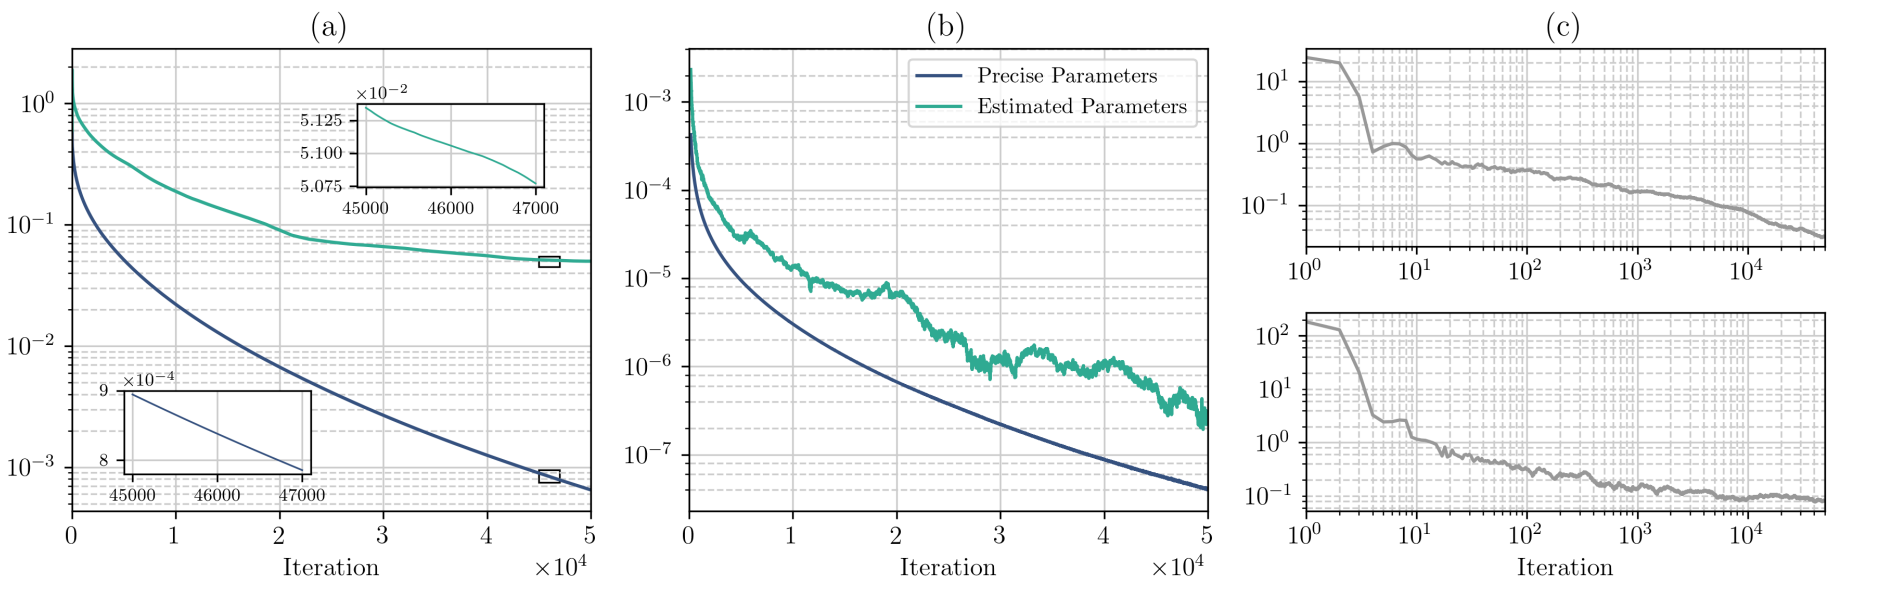
\includegraphics[scale=0.43]{Fig_1.png}}
\caption{Продуктивність Алгоритму 3 з точним вирішувачем. (a) Нормовані відстані до справжньої рівноваги за Нешем, тобто $\frac{1}{N} \sum_{i \in \mathcal{N}}\|y_{i}^{i(k)}- y_{i}^{i *}\|_{2} /\|y_{i}^{i *}\|_{2}$. (b) Відносна довжина кроку оновлення на кожній ітерації, тобто $\frac{1}{N} \sum_{i \in \mathcal{N}}\|y_{i}^{i(k +1)}-y_{i}^{i(k)}\|_{2}/\|y_{i}^{i(k)}\|_{2}$. (c:1) Нормовані відстані оцінених ваг до точних ваг, тобто $\frac{1}{N} \sum_{i \in \mathcal{N}}(\sum_{j \in \mathcal{ N}_{i}^{+}} \| \hat{P}_{j i}^{(k)} \hat{H}_{j}^{(k)} - P_{j i}^{*} H_{j}^{*} \|_{2}^{2})^{1 / 2} /(\sum_{j \in \mathcal{ N}_{i}^{+}}\|P_{j i}^{*} H_{j}^{*}\|_{2}^{2})^{1 / 2}$. (c:2) Нормовані відстані оцінених зміщень до точних зміщень, тобто $\frac{1}{N} \sum_{i \in \mathcal{N}}|b_{i}^{(k )}-b_{i}^{*}| /|b_{i}^{*}|$.}
\label{Fig1}
\end{figure}

\begin{figure}[]
\left{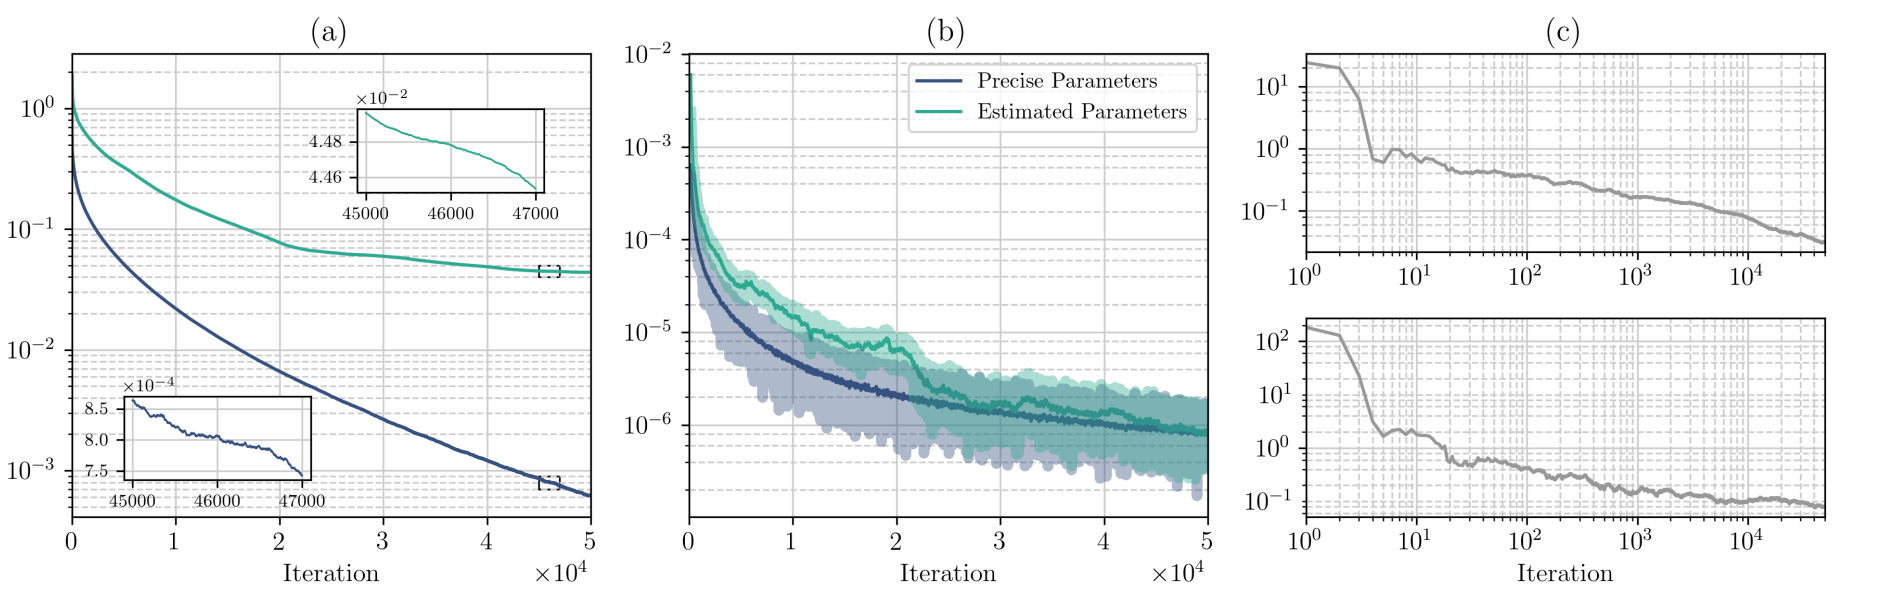
\includegraphics[scale=0.43]{Fig_2.png}}
\caption{Продуктивність Алгоритму 3 з неточним вирішувачем. (a) Нормовані відстані до справжньої рівноваги за Нешем, тобто $\frac{1}{N} \sum_{i \in \mathcal{N}}\|y_{i}^{i(k)}- y_{i}^{i *}\|_{2} /\|y_{i}^{i *}\|_{2}$. (b) Відносна довжина кроку оновлення на кожній ітерації, тобто $\frac{1}{N} \sum_{i \in \mathcal{N}}\|y_{i}^{i(k +1)}-y_{i}^{i(k)}\|_{2} /\|y_{i}^{i(k)}\|_{2}$. Товста та напівпрозора лінія позначає реальні коливання показника, а суцільна та тонка лінія відображає прості ковзні середні метрики з розміром вікна 80. (c:1) Нормовані відстані оцінених ваг до точної ваги, тобто $\frac{1}{N} \sum_{i \in \mathcal{N}}(\sum_{j \in \mathcal{N}_{i}^{+}} \|\hat{P}_{j i}^{(k)} \hat{H}_{j}^{(k)}-P_{j i}^{*} H_{j}^{*}\|_{2}^{2})^{1 / 2} /(\sum_{j \in \mathcal{N}_{i}^{+}}\|P_{ j i}^{*} H_{j}^{*}\|_{2}^{2})^{1 / 2}$. (c:2) Нормовані відстані оцінених зміщень до точних зміщень, тобто $\frac{1}{N} \sum_{i \in \mathcal{N}}|b_{i}^{(k )}-b_{i}^{*}| /|b_{i}^{*}| .$}
\label{Fig2}
\end{figure}

\subsubsection*{Симуляція результатів}\label{pr}
У грі грають $N=10$ гравців. Граф зв’язку складається з неорієнтованого кола та 10 випадково вибраних ребер. Кожна локальна допустима множина $\mathcal{X}_{i}$ є прямим добутком інтервалів $n_{i}$, тобто $\mathcal{X}_{i} := \prod_{j=1}^{n_{i}}[0, \mathcal{X}_{i j \max }]$. Пов'язані параметри витягуються рівномірно з відповідних інтервалів. Розмір $n_{i}$ задовольняє $n_{i} \sim U\{3,4,5\}$, та кожна верхня межа локальних допустимих множин задовольняє $\mathcal{X}_{i j \max } \sim U[10,20]$. Встановлюємо базову ціну $b_{0}=50$ та $b_{i}^{*} \sim U[3,7]$. Виробнича вартість $f_{i}$ містить кожну позицію $Q_{i}$, вибрану з $U[4.4,4.6]$, та кожну позицію $q_{i}$, вибрану з $U[1,1.2]$. Записи матриці суміжності $P^{*}$ рівномірно витягуються з $U[0.8,1]$ та пізніше упорядковуються, щоб мати одиничну суму по кожному рядку. Кожен запис невідомих ваг $H_{i}^{*}$ вибирається з $U[0.8,4.5]$. Кожен випадковий шум $\xi_{i}$ має усічений Гаусовий розподіл із математичним сподіванням нуль та стандартним відхиленням $0.5$. Гравець $i$ обирає кожен запис свого випадкового вектора дослідження з $U\left[-\delta_{i},+\delta_{i}\right]$, де $\delta_{i}=$ $\frac{0,01 }{2 \sqrt{n_{i}}} \min \left\{\mathcal{X}_{i j \max}: j=1, \ldots, n_{i}\right\}$. Параметри $\rho$ та $\tau$ правильно підібрані таким чином, що $\mathbb{T}$ є максимально монотонним, а $\Phi$ додатно визначеним.

Ми встановлюємо послідовність $(\gamma^{(k)})_{k \in \mathbb{N}}$ як $\gamma^{(k)}=k^{-0,501}$. Оскільки формулювання цілей очікуваного значення в цей приклад є негайним, спочатку розглянемо наступні два випадки, які включали точний розв'язок: (i) пошук рівноваги за Нешем з точними параметрами (\ref{iterat}); (ii) навчання пошуку рівноваги за Нешем з оцінюваними параметрами (Алгоритм 3). Ефективність запропонованого алгоритму проілюстрована на Рис. \ref{Fig1}. Потім досліджуємо два вищезазначені випадки з неточним розв'язанням, описаним в Алгоритмі 5 з $T_{i}^{(k)}:=\lceil 0.01 k\rceil+ 10$. Ефективність цієї заміни проілюстрована на Рис. \ref{Fig2}. Перші 150 точок на Рис. \ref{Fig1} (b) і Рис. \ref{Fig2} (b) відкидаються, щоб краще проілюструвати тенденції протягом ітерацій. В обох випадках ми бачимо, що нормовані відстані до справжньої рівноваги швидко зменшуються на перших $2 \x 10^{4}$ ітераціях, хоча в експериментах із використанням неточного вирішувача відносні довжини кроку оновлення різко коливаються. Однак, швидкість збіжності до справжньої рівноваги сповільнюється в міру проходження ітерацій, в основному переважають швидкості збіжності оцінених параметрів до їх істинної відповідності. Залишається цікавим питання строгого виведення верхньої межі для швидкості збіжності Алгоритму 3 та дослідження її залежності від розмірів невідомих параметрів, а також від розмірів векторів рішення.

\subsubsection{Інші мотиваційні приклади мережевих ігор}

\subsubsection*{Приклад (Когнітивні радіосистеми)}

Розглянемо проблему проєктування когнітивної радіосистеми, передача якої здійснюється через частотно-селективні канали з одним входом і одним виходом. Він складається з $N^{p}$ первинних користувачів, $N$ вторинних користувачів та $n^{s}$ доступних йому частот. Ці $N$ вторинних користувачів, індексовані $\mathcal{N} := \{1, \ldots, N\}$, беруть участь у грі розподілу частотних ресурсів, де кожен вторинний користувач $i$ змагається один з одним, щоб максимізувати власну швидкість інформації шляхом визначення вектора розподілу потужності $x_{i} \in \mathbb{R}^{n_{i}^{s}}$ над доступними йому частотам $n_{i}^{s}$. Тут цільова функція кожного вторинного користувача $i \in \mathcal{N}$ часто може бути виражена як:
\begin{equation}
    \begin{align}
&\mathbb{J}_{i}(x_{i}; x_{i}^{+}, w_{i}^{*}) := \mathbb{E}_{\xi_{ i}}[-\sum_{s \in \mathcal{S}_{i}} J_{i, s}(x_{i}; x_{i}^{+}, w_{i} ^{*}, \xi_{i}(s))], \text { де } \\
&J_{i, s}(x_{i}; x_{i}^{+}, w_{i}^{*}, \xi_{i}(s)):=\log ( 1+\frac{|H_{i i}(s)|^{2}[x_{i}]_{s}}{\sigma_{i}^{2}(s) +\sum_{s \in \mathcal{S}_{j}, j \neq i}|H_{i j}(s)|^{2}[x_{j}]_ {s}+\xi_{i}(s)})
\end{align}
\end{equation}
де $\mathcal{S}_{i}:=\left\{1, \ldots, n_{i}^{s}\right\}$ — набір індексів для частот, доступних для вторинного користувача $i, \sigma_ {i}^{2}(s)$ позначає потужність теплового шуму над частотою $s, H_{i j}(s)$ це функція передачі каналу між вторинним передавачем $j$ та приймачем $i,\left [x_{i}\right]_{s}$ являє собою запис вектора $x_{i}$, пов'язаного з рішенням про розподіл потужності частоти $s$, а $\xi_{i}(s)$ представляє невизначеність у реалізацію мети. У цій мережевій грі топологія зв'язку побудована таким чином, що кожен вторинний користувач $i$ може спілкуватися з іншими вторинними користувачами, які мають прямий конкуруючий інтерес у зайнятті певної частоти $s \in \mathcal{S}_{i}$, тобто $\mathcal{N}_{i}^{+}:=\{j \in \mathcal{N} \mid(j, i ) \in \mathcal{E}\}$ задовольняє $\mathcal{N}_{i}^{+}=\{j \in \mathcal{N} \mid \exists s \in \mathcal{S }_{i}.$ с.т. $s \in$ $\left.\mathcal{S}_{j}, j \neq i\right\}$. Припустимо, що $\left|H_{i i}(s)\right|^{2}$ доступний для кожного вторинного користувача $i$, тоді як $\sigma_{i}^{2}(s)$ та $\{|H_{i j}(s)|^{2}\}_{j \in \mathcal{N}_{-i}}$ – це невідомі параметри, які слід вивчити, тобто $ w_{i}^{*}:=[\sigma_{i}^{2}(s) ;\left[H_{i j}(s)\right]_{j \in \mathcal{N}_ {-i}}]_{s \in \mathcal{S}_{i}}$. Передбачається, що пов’язана можлива область $\mathcal{W}_{i}$ є деяким невід’ємним набором коробок.

Використовуємо $Q_{p i}(s)$ для представлення функції передачі каналу між вторинним передавачем $i$ та первинним приймачем $p$ через частоту $s$, а $I_{p i}^{\text {tot }}$ максимальні перешкоди, які дозволено створювати вторинному користувачу $i$ на первинному приймачі $p$ по всьому спектру. Локальна можлива множина кожного вторинного користувача $i$ визначається наступним чином:
\begin{equation}\label{thirdseven}
    \begin{align}
    \mathcal{X}_{i} := \left\{x_{i} \in \mathbb{R}^{n_{i}^{s}} \mid \mathbf{0} \leq x_{i} \leq b_{i}, \mathbf{1}_{n_{i}^{s}}^{T} x_{i} \leq \bar{\kappa} \cdot \mathbf{1}_{n_{ i}^{s}}^{T} b_{i},\right. \\
    \left.\sum_{s \in \mathcal{S}_{i}}\left|Q_{p i}(s)\right|^{2}\left[x_{i}\right]_{s} \leq I_{p i}^{t o t}, \forall p\right\}
    \end{align}
\end{equation}
де $b_{i} \in \mathbb{R}^{n^{s}}$ — вектор із додатними записами, а $\bar{\kappa} \in(0,1)$ — деяка задана константа. На додаток до локальних обмежень у (\ref{thirdseven}), можливо, що за деяких обставин вектор розподілу потужності $\left\{x_{i}\right\}$ усіх вторинних користувачів повинен разом задовольняти наступним глобальним обмеженням для $p = 1, \ldots, N^{p}$:
\begin{equation}
    \begin{aligned}
    \sum_{i \in \mathcal{N}, s \in \mathcal{S}_{i}}\left|Q_{p i}(s)\right|^{2}\left[x_{i}\right]_{s} \leq I_{p}^{\text {peak}}(s), \forall s=1, \ldots, n^{s}, \\
    \sum_{i \in \mathcal{N}} \sum_{s \in \mathcal{S}_{i}}\left|Q_{p i}(s)\right|^{2}\left[x_{i}\right]_{s} \leq I_{p}^{\text {tot }},
    \end{aligned}
\end{equation}

де $I_{p}^{\text {peak }}(s)$ і $I_{p}^{\text {tot }}$ представляють максимальні перешкоди, дозволені для створення всім вторинним користувачам на первинному приймачі $p$ по частоті $k$ та всьому спектру відповідно.

\clearpage
\subsection{Порівняння алгоритмів}

У грі грають $N=10$ гравців. Гравці є виробниками деякої продукції, одиниця товару якою має певну початкову ціну $x_i$. Ціна формується з витрат виробника на одиницю товару та доходу, в задачі розглядаємо собівартість товару як 0, та максимальну ціну що може встановити виробник як 1.

Рівновагою Неша у даній грі є ситуація коли всі гравці продають товар по собівартості. Якщо припустити, що всі гравці продаватимуть товар по ненульовій ціні, то кожен гравець може змінити свою ціну на нижчу за мінімальну серед всіх гравців та переманити велику частку покупців.

Ціна за товар визначається випадково, як $x_i = 0.75 + 0.25 \cdot U(0,1)$.

Функція корисності гравців має вигляд $f_i(x_i,\overline{x}_i)=\frac{3}{4}\|x_i-x_i^*\|^2+(\overline{x}_i+0.5) \cdot x_i~,$

Матриця ваг $W = \{w_{ij}\}$ задається так
\begin{eqnarray}
w_{ij} =
\begin{cases}
\frac{1}{18}, & i\neq j\\
0.5, &  i = j
\end{cases}
\end{eqnarray}

Далі кожен гравець починає діяти згідно з алгоритмом (\ref{alg1}, \ref{alg2}, \ref{alg3}). 

\begin{figure}[h]
\centering
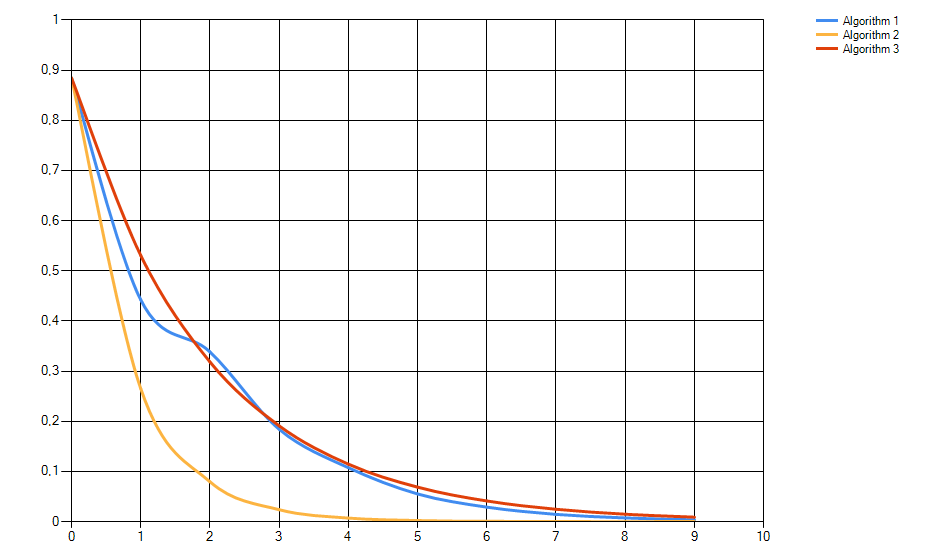
\includegraphics[scale=0.8]{Screenshot_1.png}
\caption{Середнє значення ціни між всіма гравцями впродовж часу.}
\end{figure}

\noindentСимуляція була розрахована на\\
ASUS Vivobook S13 S330,\\
Операційна система: Windows 11,\\
Процесор: Intel(R) Core(TM) i5-8265U CPU @ 1.60GHz 1.80 GHz,\\
Оперативна пам'ять: 8,00 ГБ,\\
Тип системи	64-розрядна.\\
Код був написаний та налагоджений у середовищі виконання <<Microsoft .NET SDK 5.407 (x64) from Visual Stodio>> з використанням бібліотеки\\ <<System.Windows.Forms>> та інших наведених в Додатку за допомогою мови C$\#$.



\clearpage
\section{Висновки}

На закінчення слід особливо підкреслити, що теорія ігор є дуже складною сферою знань. При поводженні з нею треба дотримуватися правил та бути дуже обережним, чітко знати межі її застосування. Аналіз і консультації на основі теорії ігор через їх складності рекомендуються лише для особливо важливих проблемних областей. Однак застосування теорії ігор полегшує нам розуміння суті того, що відбувається, а багатогранність даного розділу науки дозволяє нам успішно використовувати методи й властивості цієї теорії в різних областях нашої діяльності.

Теорія ігор прищеплює людині дисципліну розуму. Від особи, яка приймає рішення, вона вимагає систематичного формулювання можливих альтернатив поведінки, оцінки їх результатів, і найголовніше — дослідження поведінки інших. Людина, знайома з теорією ігор, рідше вважає інших дурнішими за себе, і тому уникає багатьох непробачних помилок. Однак теорія ігор не може, та й не розрахована на те, щоб надати рішучості, наполегливості в досягненні цілей, всупереч невизначеності та ризику. Знання основ теорії ігор не дає нам явного виграшу, але оберігає нас від звершення дурних і непотрібних помилок.

В останні роки значення теорії ігор істотно зросло в багатьох областях економічних і соціальних наук. В економіці вона застосовна не тільки для вирішення загальногосподарських завдань, а й для аналізу стратегічних проблем підприємств, розробок організаційних структур і систем стимулювання.

Дисципліна створена для математичного вирішення завдань економічного і соціального походження, не може в цілому зводитися до класичних математичних теорій, створених для вирішення фізичних і технічних завдань. Однак в різних конкретних питаннях теорія ігор широко використовує різноманітні класичні математичні методи. Крім цього, вона пов'язана з рядом математичних дисциплін внутрішнім чином. У теорії ігор систематично і по суті вживаються поняття теорії ймовірностей. Її мовою можна сформулювати більшість завдань математичної статистики.

У даній роботі я намагався донести основні поняття теорії ігор, дослідити алгоритми пошуку рівноваги та їх вплив на економічну сферу. Як було зазначено алгоритми застосовуються на одному типі задач, деталі який можуть відрізнятися, тому використання того чи іншого алгоритму визначається насамперед способом формалізації реальної ситуації на ринку.

Кожен з наведених алгоритмів може бути застосований в економічній сфері, на мою думку найбільш застосовним до реального світу є алгоритм (\ref{alg3}), але він потребує найбільш детальної формалізації ринкової ситуації для точного розв'язку.

\clearpage
\begin{thebibliography}{05}
\addcontentsline{toc}{section}{\refname}
{\small

\bibitem{Gubko} М.~Губко, Д.~Новиков, Теория игр в управлении организационными системами, М: Синтег, 2002~г.

\bibitem{Danilov} В.~Данилов, Лекции по теории игр. М.: препринт РЭШ, 2002

\bibitem{Zaharov} А.~Захаров, Теория игр в общественных науках. М.: препринт НИУ ВШЭ, 2014

\bibitem{Mazalov} В.~Мазалов, Математическая теория игр и приложения, Санкт-Петербург, Лань, 2010~г.

\bibitem{Menshikov} И.~Меньшиков, Лекции по теории игр и экономическому моделированию, М.: Контакт Плюс 2010~г.

\bibitem{Shen} А.~Шень, Игры и стратегии с точки зрения математики. Москва, Издательство МЦНМО 2018

\bibitem{Neyman} Дж.~фон~Нейман, Э.~Моргенштерн, Теория игр и экономическое поведение. М. : Наука, 1970. 708~с.

\bibitem{Osborne} M.~Osborne, A.~Rubinstein, A Course in Game Theory, MIT press, Cambridge, MA, 1994.

\bibitem{Cite2} M. Bianchi, S. Grammatico, <<Fully distributed nash equilibrium seeking over time-varying communication networks with linear convergence rate>>, IEEE Control Systems Letters, vol. 5, no. 2, pp. 499–504, 2021.

\bibitem{Cite22}\label{Cite22} S.~Liang, P.~Yi, Y.~Hong, <<Distributed Nash equilibrium seeking for aggregative games with coupled constraints>>, Automatica, vol. 85, pp. 179–185, 2017.

\bibitem{Cite3} J. Koshal, A. Nedic, U. Shanbhag, <<Distributed algorithms for aggregative games on graphs>>, Operations Research, vol. 64, no. 3, pp. 680–704, 2016.

\bibitem{Cite21} C.~De~Persis, S.~Grammatico, <<Distributed Nash equilibrium seeking by a consensus based approach>>, IEEE Trans. on Automatic Control, vol. 62, no. 9, pp. 4811–4818, 2017.

\bibitem{Article1} C.~De~Persis, S.~Grammatico <<Continuous-time integral dynamics for aggregative game equilibrium seeking>>

[Електронний ресурс]: arXiv preprint arXiv:1803.10448v1, 2018

URL: \url{https://arxiv.org/pdf/1803.10448.pdf}

\bibitem{Cite1} R.~Zhu, J.~Zhang, K.~You, T.~Basar, <<Asynchronous networked
aggregative games>>

[Електронний ресурс]: arXiv preprint arXiv:2101.08973, 2021.

URL: \url{https://arxiv.org/pdf/2101.08973.pdf}

\bibitem{Article2} R.~Zhu, J.~Zhang, K.~You <<Networked Aggregative Games with Linear Convergence>>

[Електронний ресурс]: arXiv preprint arXiv:2105.05465v1, 2021

URL: \url{https://arxiv.org/pdf/2105.05465.pdf}

\bibitem{Article3}\label{Article3} Y. Huang, J. Hu <<Distributed Stochastic Nash Equilibrium Learning in Locally Coupled Network Games with Unknown Parameters>>

[Електронний ресурс]: arXiv preprint arXiv:2204.00100v2, 2022

URL: \url{https://arxiv.org/pdf/2204.00100.pdf}
}
\end{thebibliography}

\clearpage
\section*{Додаток}
\addcontentsline{toc}{section}{Додаток}

\begin{minted}[fontsize=\footnotesize]{c++}

using System;
using System.Collections.Generic;
using System.Linq;
using System.Threading.Tasks;
using System.Windows.Forms;

namespace WindowsFormsApp1
{
    static class Program
    {
        [STAThread]
        static void Main()
        {
            Application.EnableVisualStyles();
            Application.SetCompatibleTextRenderingDefault(false);
            Application.Run(new Form1());
        }
    }
}

namespace WindowsFormsApp1
{
    partial class Form1
    {
        protected override void Dispose(bool disposing)
        {
            if (disposing && (components != null))
            {
                components.Dispose();
            }
            base.Dispose(disposing);
        }

        private void InitializeComponent()
        {
            System.Windows.Forms.DataVisualization.Charting.ChartArea chartArea1 = new System.Windows
            .Forms.DataVisualization.Charting.ChartArea();
            System.Windows
            .Forms.DataVisualization.Charting.Legend legend1 = new System.Windows
            .Forms.DataVisualization.Charting.Legend();
            System.Windows
            .Forms.DataVisualization.Charting.Series series1 = new System.Windows
            .Forms.DataVisualization.Charting.Series();
            System.Windows
            .Forms.DataVisualization.Charting.Series series2 = new System.Windows
            .Forms.DataVisualization.Charting.Series();
            System.Windows
            .Forms.DataVisualization.Charting.Series series3 = new System.Windows
            .Forms.DataVisualization.Charting.Series();
            this.chart = new System.Windows.Forms.DataVisualization.Charting.Chart();
            this.button = new System.Windows.
            Forms.Button();
            this.button2 = new System.Windows.
            Forms.Button();
            this.button1 = new System.Windows.
            Forms.Button();
            this.button3 = new System.Windows.
            Forms.Button();
            ((System.ComponentModel.ISupportInitialize)(this.chart)).BeginInit();
            this.SuspendLayout();
            // 
            // chart
            // 
            chartArea1.AxisX.Minimum = 0D;
            chartArea1.AxisY.Interval = 0.1D;
            chartArea1.AxisY.Maximum = 1D;
            chartArea1.AxisY.Minimum = 0D;
            chartArea1.Name = "ChartArea1";
            this.chart.ChartAreas.Add(chartArea1);
            legend1.Name = "Legend1";
            this.chart.Legends.Add(legend1);
            this.chart.Location = new System.Drawing.Point(12, 12);
            this.chart.Name = "chart";
            series1.BorderWidth = 3;
            series1.ChartArea = "ChartArea1";
            series1.ChartType = System.Windows.Forms.DataVisualization.Charting.SeriesChartType.
            Spline;
            series1.Legend = "Legend1";
            series1.LegendText = "Algorithm 1";
            series1.Name = "Series1";
            series2.BorderWidth = 3;
            series2.ChartArea = "ChartArea1";
            series2.ChartType = System.Windows.Forms.DataVisualization.Charting.SeriesChartType.
            Spline;
            series2.Legend = "Legend1";
            series2.LegendText = "Algorithm 2";
            series2.Name = "Series2";
            series3.BorderWidth = 3;
            series3.ChartArea = "ChartArea1";
            series3.ChartType = System.Windows.Forms.DataVisualization.Charting.SeriesChartType.
            Spline;
            series3.Legend = "Legend1";
            series3.LegendText = "Algorithm 3";
            series3.Name = "Series3";
            this.chart.Series.Add(series1);
            this.chart.Series.Add(series2);
            this.chart.Series.Add(series3);
            this.chart.Size = new System.Drawing.Size(950, 577);
            this.chart.TabIndex = 0;
            this.chart.Text = "chart2";
            // 
            // button
            // 
            this.button.Location = new System.Drawing.Point(978, 26);
            this.button.Name = "button";
            this.button.Size = new System.Drawing.Size(177, 78);
            this.button.TabIndex = 1;
            this.button.Text = "Algorithm 1";
            this.button.UseVisualStyleBackColor = true;
            this.button.Click += new System.EventHandler(this.button_Click);
            // 
            // button2
            // 
            this.button2.Location = new System.Drawing.Point(978, 194);
            this.button2.Name = "button2";
            this.button2.Size = new System.Drawing.Size(177, 78);
            this.button2.TabIndex = 3;
            this.button2.Text = "Algorithm 3";
            this.button2.UseVisualStyleBackColor = true;
            this.button2.Click += new System.EventHandler(this.button2_Click);
            // 
            // button1
            // 
            this.button1.Location = new System.Drawing.Point(978, 110);
            this.button1.Name = "button1";
            this.button1.Size = new System.Drawing.Size(177, 78);
            this.button1.TabIndex = 4;
            this.button1.Text = "Algorithm 2";
            this.button1.UseVisualStyleBackColor = true;
            this.button1.Click += new System.EventHandler(this.button1_Click);
            // 
            // button3
            // 
            this.button3.Location = new System.Drawing.Point(978, 338);
            this.button3.Name = "button3";
            this.button3.Size = new System.Drawing.Size(177, 78);
            this.button3.TabIndex = 5;
            this.button3.Text = "Init";
            this.button3.UseVisualStyleBackColor = true;
            this.button3.Click += new System.EventHandler(this.button3_Click);
            // 
            // Form1
            // 
            this.ClientSize = new System.Drawing.Size(1167, 594);
            this.Controls.Add(this.button3);
            this.Controls.Add(this.button1);
            this.Controls.Add(this.button2);
            this.Controls.Add(this.button);
            this.Controls.Add(this.chart);
            this.Name = "Form1";
            ((System.ComponentModel.ISupportInitialize)(this.chart)).EndInit();
            this.ResumeLayout(false);

        }

        private System.Windows.Forms.DataVisualization.Charting.Chart chart1;
        private System.Windows.Forms.DataVisualization.Charting.Chart chart;
        private System.Windows.Forms.Button button;
        private System.Windows.Forms.Button button2;
        private System.Windows.Forms.Button button1;
        private System.Windows.Forms.Button button3;
    }
}

using System;
using System.Collections.Generic;
using System.ComponentModel;
using System.Data;
using System.Drawing;
using System.Linq;
using System.Text;
using System.Threading.Tasks;
using System.Windows.Forms;

namespace WindowsFormsApp1
{
    public partial class Form1 : Form
    {
        public Form1()
        {
            InitializeComponent();
        }
        private void Form1_Load(object sender, EventArgs e)
        {
        }

        // Fields
        Random rnd = new Random();
        static int a = 0, b = 10, t = 0, h = 1;
        static double y = 0;

        static int N = 10;
        List<double> xs_started = new List<double>() { };

        private void init() {
            xs_started.Clear();
            for (int i = 0; i < N; i++)
            {
                xs_started.Add(0.75 + 0.25*rnd.NextDouble());
            }
        }

        private double average(List<double> xs)
        {
            y = 0;
            xs.ForEach(x => y += x);
            y /= N;
            return y;
        }

        private void button_Click(object sender, EventArgs e)
        {
            var xs = new List<double>();
            for (int i = 0; i < N; i++)
            {
                xs.Add(xs_started[i]);
            }

            var Series = this.chart.Series[0].Points;
            Series.Clear();

            for (int t = 0; t < b; t++)
            {
                y = average(xs);
                Series.AddXY(t, y);
                Alghoritm1(xs);
            }
        }

        private void button1_Click(object sender, EventArgs e)
        {
            var xs = new List<double>();
            for (int i = 0; i < N; i++)
            {
                xs.Add(xs_started[i]);
            }

            var vs = new List<double>();
            for (int i = 0; i < N; i++)
            {
                vs.Add(xs_started[i]);
            }

            for (int i = 0; i < N; i++)
            {
                W.Add(new List<double>());
                for (int j = 0; j < N; j++)
                {
                    if (i == j)
                    {
                        W[i].Add(1 - delta * d);
                    }
                    else
                    {
                        W[i].Add(delta);
                    }
                }
            }

            var Series = this.chart.Series[1].Points;
            Series.Clear();

            for (int t = 0; t < b; t++)
            {
                y = average(xs);
                Series.AddXY(t, y);
                Alghoritm2(xs, vs);
            }
        }

        private void button2_Click(object sender, EventArgs e)
        {
            var xs = new List<double>();
            for (int i = 0; i < N; i++)
            {
                xs.Add(xs_started[i]);
            }

            var Series = this.chart.Series[2].Points;
            Series.Clear();

            for (int t = 0; t < b; t++)
            {
                y = average(xs);
                Series.AddXY(t, y);
                Alghoritm3(xs);
            }
        }

        private void button3_Click(object sender, EventArgs e)
        {
            init();
        }

        double sigma = 0;
        private void Alghoritm1(List<double> xs)
        {
            for (int i = 0; i < xs.Count; i++)
            {
                xs[i] = 1 / 2 * 1.5 * Math.Pow((xs[i] - (0.25 + 0.5 * rnd.NextDouble())), 2) 
                + (sigma + 0.5) * xs[i];
            }
            sigma = 0.6*(-sigma + average(xs));
        }

        static double d = N - 1, delta = 0.5 / d;
        static List<List<double>> W = new List<List<double>>();
        private void Alghoritm2(List<double> xs, List<double> vs)
        {
            var xs_ = new List<double>();
            for (int i = 0; i < N; i++)
            {
                xs_.Add(xs[i]);
            }

            var xs_prev = new List<double>();
            for (int i = 0; i < N; i++)
            {
                xs_prev.Add(xs[i]);
            }

            var vs_ = new List<double>();
            for (int i = 0; i < N; i++)
            {
                vs_.Add(xs[i]);
            }

            for (int i = 0; i < N; i++)
            {
                vs_[i] = 0;
                for (int j = 0; j < N; j++)
                {
                    vs_[i] += W[i][j] * vs[j];
                }

                double prod = 0;
                for (int j = 0; j < N; j++)
                {
                    prod *= xs_[j] - 0.1 * (xs[i] + vs_[i])/2;
                }
                xs_[i] = prod;

                xs[i] = 3*(xs[i] + 0.9 * (xs_[i] - xs[i]));
                vs[i] = vs_[i] + xs[i] - xs_prev[i];
            }

        }

        private void Alghoritm3(List<double> xs)
        {
            var xs_ = new List<double>();
            for (int i = 0; i < N; i++)
            {
                xs_.Add(xs[i]);
            }

            var xs_prev = new List<double>();
            for (int i = 0; i < N; i++)
            {
                xs_prev.Add(xs[i]);
            }

            for (int i = 0; i < N; i++)
            {

                double prod = 0;
                for (int j = 0; j < N; j++)
                {
                    prod *= xs_[j] - 0.1 * (xs[i]) / 2;
                }
                xs_[i] = prod;

                xs[i] =(xs[i] + 0.9 * (xs_[i] - xs[i]));
            }
        }


\end{minted}

\end{document}